%============================================%
% Official template for CLICdp notes.
%
% Updated: 22.06.2014
% Christian Grefe (christian.grefe@cern.ch)
%============================================%

\documentclass[11pt,a4paper]{scrartcl}

% Defines default style and includes several useful packages
\usepackage{CLICdp}

% Useful macros for writing CLICdp notes
\usepackage{CLICdp_definitions}

% Add your packages here
%\usepackage{MyPackage}


%============================================%
% Set up the title page
%============================================%

% Set the title of the note
\title{Measurement of the H${\rightarrow}$WW* Branching Ratio at 1.4TeV With CLIC ILD Using the WW*${\rightarrow}$qql$\nu$ Final State }

% Set the CLICdp note number
\clicdpnote{2015}{001}  % public notes
%\clicdppub{2014}{001}  % journal articles
%\clicdpconf{2014}{001}  % conference proceedings
%\clicdpdraft{2014}{001}  % draft versions for circulation 

% Set the publication date
\date{\today}
%\date{\formatdate{18}{6}{2014}}

% Define the authors and their institutes, they will appear exactly in the order as they are added
% Footnotes can be added using the \thanks command
%\addauthor{A.~Winter}{\institute{1}\institute{2}}
\addauthor{A.~Winter}{\institute{1}}
\addauthor{N.~Watson}{\institute{1}}
%\addauthor{Initials.~Name\thanks{corresponding.author@cern.ch}}{\institute{1}}

\addinstitute{1}{University of Birmingham, United Kingdom}
%\addinstitute{2}{University, Country}
%\addinstitute{3}{Other University, Country}

% Add "On behalf of ... (optional)"
\onbehalfof{the CLICdp collaboration}

% Define an abstract for the note 
\abstract{This note summarises a study to evaluate the potential to measure the H$\rightarrow$WW$^*$ branching fraction at CLIC, at 1.4TeV centre-of-mass energy, using the WW$\rightarrow$qql$\nu$ channel. We will discuss the approach to reconstructing the final state and the methods used to separate signal events from backgrounds. The expected statistical precision on the product branching fraction, $\delta(\sigma_{H\nu\nu}$ x BR(H$\rightarrow$WW$^*$)), is found to be 1.3\% for an integrated luminosity of 1.5ab$^{-1}$.}

% Add comments to the title page (optional)
%\titlecomment{Talk presented at CONFERENCE, PLACE, COUNTRY, 16--19 June 2014}
\titlecomment{This work was carried out in the framework of the CLICdp collaboration}

% Uncomment this line to remove the stamp with the CLICdp note number from the top right corner
% of the title page
%\notitlestamp


%============================================%
% Bibliography
%============================================%

% define the list of bibliography data files
%\addbibresource{./examples/bibliography.bib}
\addbibresource{./bibliography/bibliography.bib}


%============================================%
% Search path for images
%============================================%

\graphicspath{ {./logos/}{./figures/} }


%============================================%
% Options
%============================================%

% Uncomment this line for a draft version. Adds a watermark and a timestamp
%\draftdocument

% Uncomment this line to change all link colours to black
%\nocolourlinks


%============================================%
% Start of the actual document
%============================================%

\begin{document}

% generates the title page
\titlepage

% include source for sections
\chapter{Conclusion}

With the growing need to decide upon which future colliders should be built to ensure a smooth transition post LHC, it is vital that the relative merits of each proposed collider are examined. Here we have presented the potential impact that a lepton collider such as \ac{CLIC} can have on precision measurmements of the standard model. In the Higgs sector we have shown how the combination of several measurements can provide access to model independent measurements of the Higgs couplings, something not possible at hadron colliders. In particular we have shown how one of these measurements, $\sigma_{H\nu\bar{\nu}} \times BR(H\rightarrow WW^*)$, might be performed at 1.4 TeV using the semileptonic decay channel and collecting 1.5 ab$^{-1}$ of data. This yielded an expected precision of: \\[10pt]\centerline{\large{$\delta\sigma_{H\nu\nu}$ x BR(H$\rightarrow$WW$^*$) = 1.34\%$_{(Stat)} \oplus$ 1.37\%$_{(Syst)}$}} \\[10pt] Combining this with measurements performed with the fully hadronic channel shows an expected statistical precision of 1.0\%, typical of what can be expected for many measurements of Higgs properties at \ac{CLIC}.

\begin{table}[t]
  \centering
  \begin{tabular}{l|c|c}
    \toprule
    Energy (GeV) & $A_{FB}^t$ $\pm$ Stat. $\oplus$ Syst. & $\sigma$  $\pm$ Stat. $\oplus$ Syst.   \\
    \midrule
    \midrule
    \multicolumn{3}{l}{ P(e$^-$)=-80\%}\\
    \midrule
    $>=$1200   & 0.563 $\pm$ 0.018 $\oplus$ 0.015 & 18.41 $\pm$ 0.37 $\oplus$ 0.29\\
    \midrule
    900-1200   & 0.546 $\pm$ 0.034 $\oplus$ 0.028 & 11.01 $\pm$ 0.38 $\oplus$ 0.31\\
    \midrule
    400-900    & 0.458 $\pm$ 0.081 $\oplus$ 0.032 & 16.56 $\pm$ 1.31 $\oplus$ 0.48\\
    \midrule
    \midrule
    \multicolumn{3}{l}{ P(e$^-$)=+80\%}\\
    \midrule
    $>=$1200  & 0.621 $\pm$ 0.024 $\oplus$ 0.016 & 9.84 $\pm$ 0.28 $\oplus$ 0.14\\
    \midrule
    900-1200  & 0.588 $\pm$ 0.045 $\oplus$ 0.027 & 5.87 $\pm$ 0.29 $\oplus$ 0.14\\
    \midrule
    400-900   & 0.514 $\pm$ 0.105 $\oplus$ 0.034 & 8.63 $\pm$ 0.83 $\oplus$ 0.19\\
    \bottomrule
  \end{tabular}
  \caption{Final summary of the expected precisions attainable from the $t\bar{t}$ analysis.}
  \label{conlusiontable}
\end{table}

A study measuring the top forward backward asymmetry and $t\bar{t}$ cross section was also shown as a means of probing the ttX vertex for hints of \ac{BSM} physics contributions. This study was performed under the assumption that \ac{CLIC} would operate with an even luminsoity split between operation with an electron beam polarization of +80\% and -80\%. Due to the energy and polarization dependence of $A_{FB}^t$ and $\sigma_{t\bar{t}}$ and the presence of a large tail in the energy spectrum of collisions at \ac{CLIC}, the analysis was performed in six bins corresponding to the combinations of two polarization states and three energy ranges to maximise the information extracted. Event reconstruction and selection was performed using techniques based on fat jet and jet substructure which have not been implemented in a lepton collider before. Ultimately the final results were extracted by performing a second order polynomial fit to the distribution of the top production angle. The resulting uncertainties for each bin are shown in \reftab{conlusiontable} and are found to be approximately an order of magnitude better than what is seen at the \ac{LHC}\cite{Bai:2011uk}. A detailed study of various systematic effects revealed that the in all cases the uncertainty is dominated by the statistical component with the dominant systematic contributions for the cross section and $A_{FB}^t$ coming from the background normalization and bias introduced during efficiency corrections respectively. In future these results will be combined with measurements from other top studies performed by \ac{CLIC} to evaluate the precision to which the electroweak form factors of the ttX can be measured.

Lastly we have examined the possibility for using a \ac{DECAL} at the \ac{ILC} as an alternative to the analgue SiW calorimeter. Such a device would use \ac{CMOS} \ac{MAPS} technology to provide an ultra high granularity capable of measuring every particle present within an \ac{EM} shower providing potential benefits for use with particle flow techniques and potential cost reductions. The resolution of a \ac{DECAL} was found to be dominated by two competing effects. At low energy boundary crossings dominate leading to a worse performance for designs based on narrower, deeper pixels. For higher energy saturation occurs as the EM shower becomes denser than the detectors granularity leading to worse performance for wider pixels. When using DigiMAPS to apply additional levels of realism such as charge diffusion, dead space, noise, threshold spreads and clustering it was found that the clustering helped mitigate the impact of boundary crossings leading to a general performance for narrow pixels thin pixels. For the typical enegy scale of the \ac{ILC} the optimal piuxel desgin was found to occur when using 30 $\mu m$ pitch, 12 $\mu m$ epi thickness pixels. This design yielded an energy resolution of:

\begin{equation}
  \frac{\sigma_E}{E}=\frac{16.1\%}{\sqrt{E}} \oplus \frac{0.5\%}{E} \oplus 0.4\%
\end{equation}

Which is comparable to the performance seen for the fully optimised design of the analogue SiW intended for use in \ac{ILD}. 


\clearpage
\section{Appendix A: Higgs Results}
\label{appendixA}
Here we show the signal and background distributions for the input variables used for training the BDT for our Higgs analysis. In all cases the plots are normalised to unity and show the raw distributions before preselection cuts are applied.

\begin{figure}[h] 
  \begin{subfigure}[]{0.5\linewidth}
    \centering
    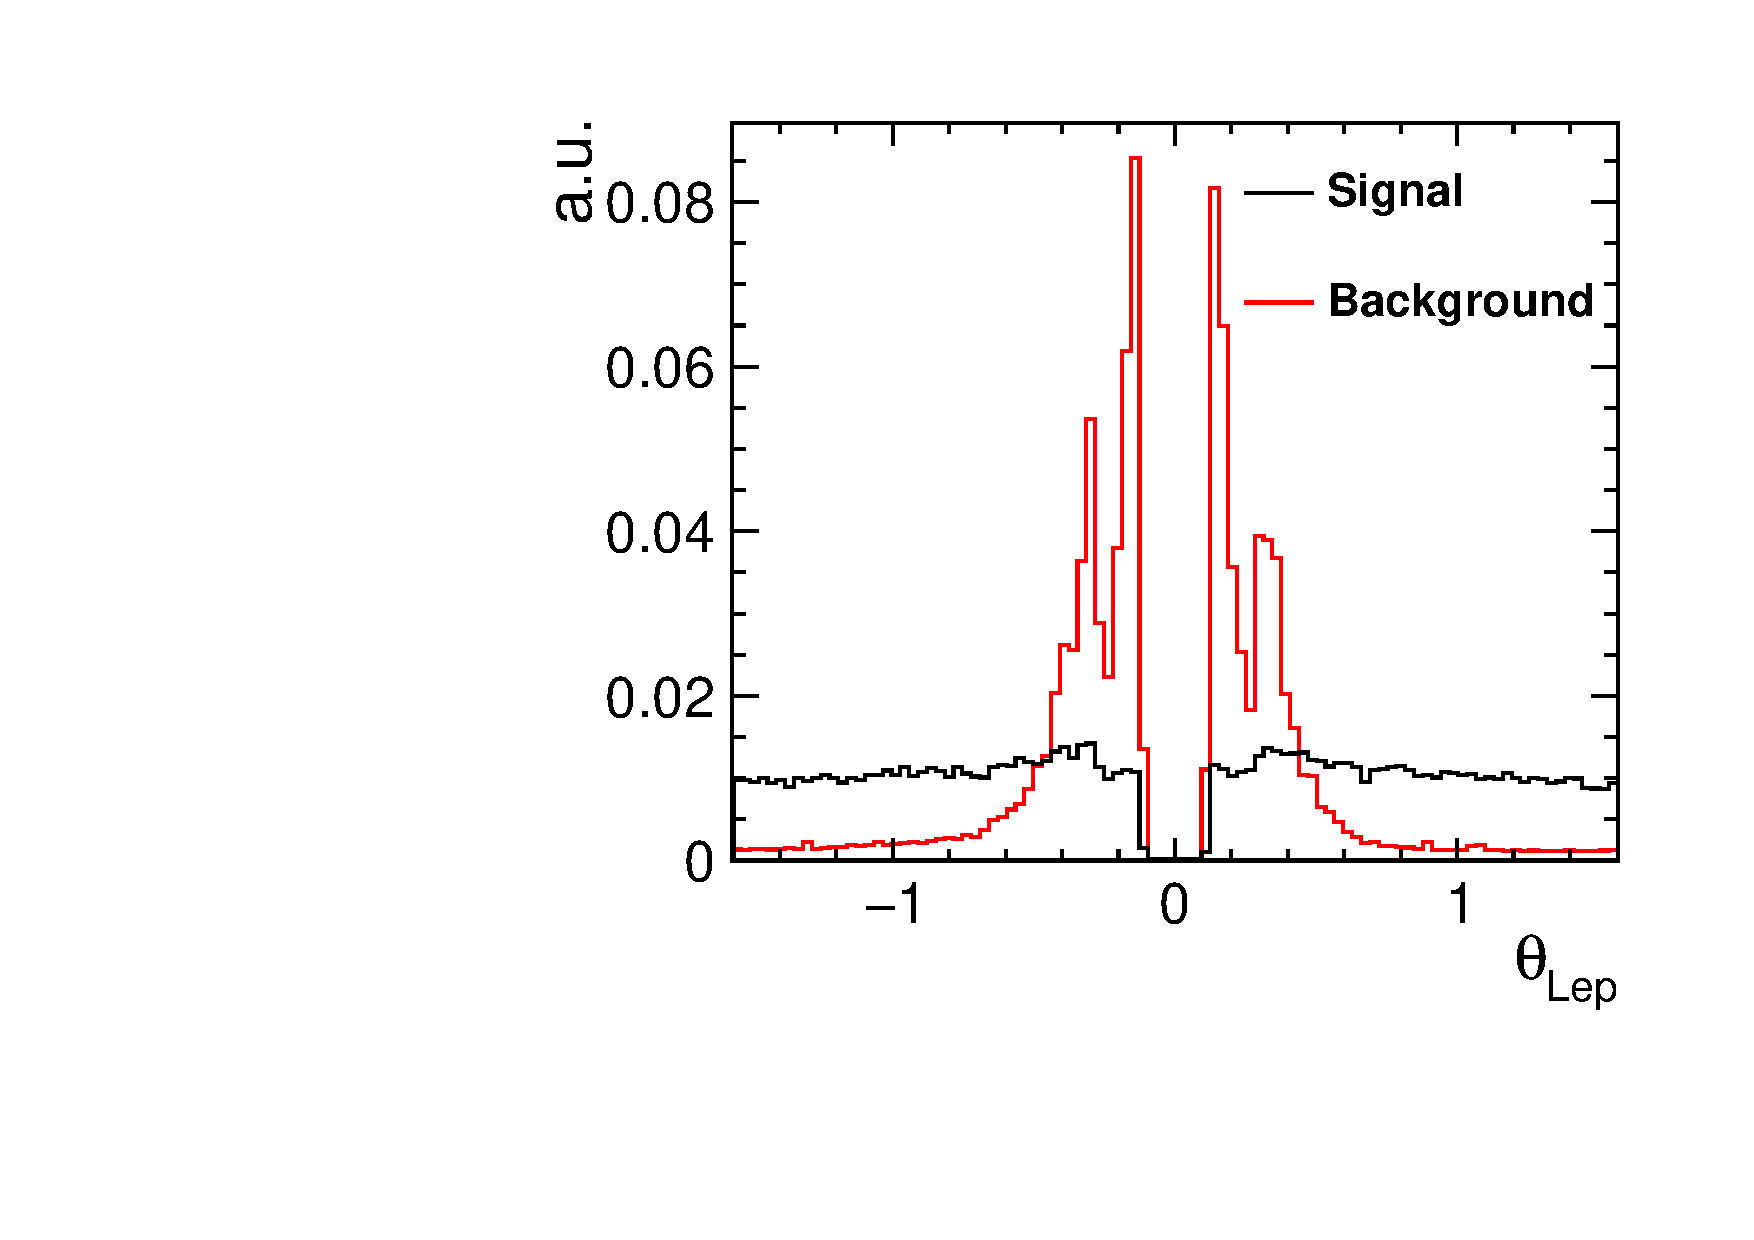
\includegraphics[width=0.75\linewidth]{Appendix/figures/DiraLep} 
    \caption{Angle of lepton relative to beam axis} 
    \vspace{4ex}
  \end{subfigure}%% 
  \begin{subfigure}[]{0.5\linewidth}
    \centering
    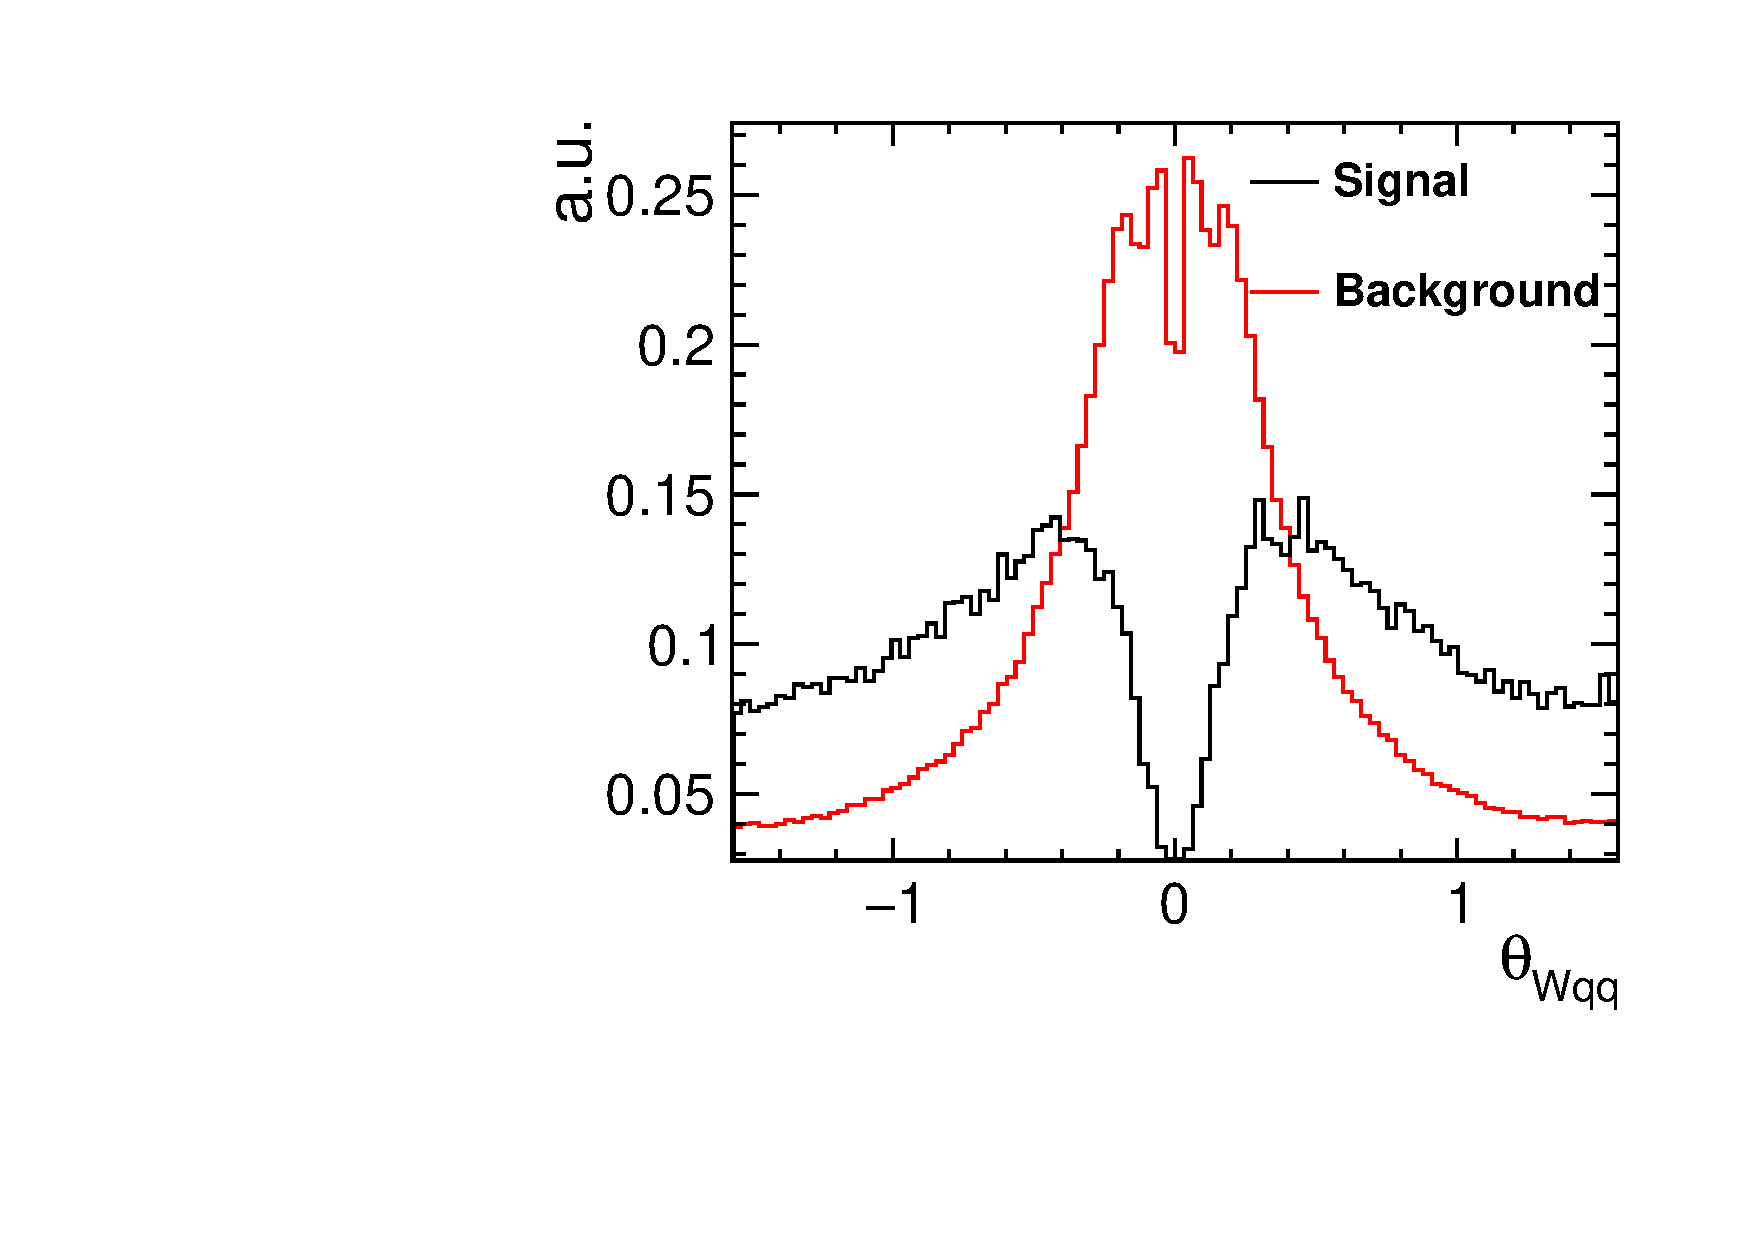
\includegraphics[width=0.75\linewidth]{Appendix/figures/DiraWqq} 
    \caption{Angle of W relative to beam axis} 
    \vspace{4ex}
  \end{subfigure}
    \begin{subfigure}[]{0.5\linewidth}
    \centering
    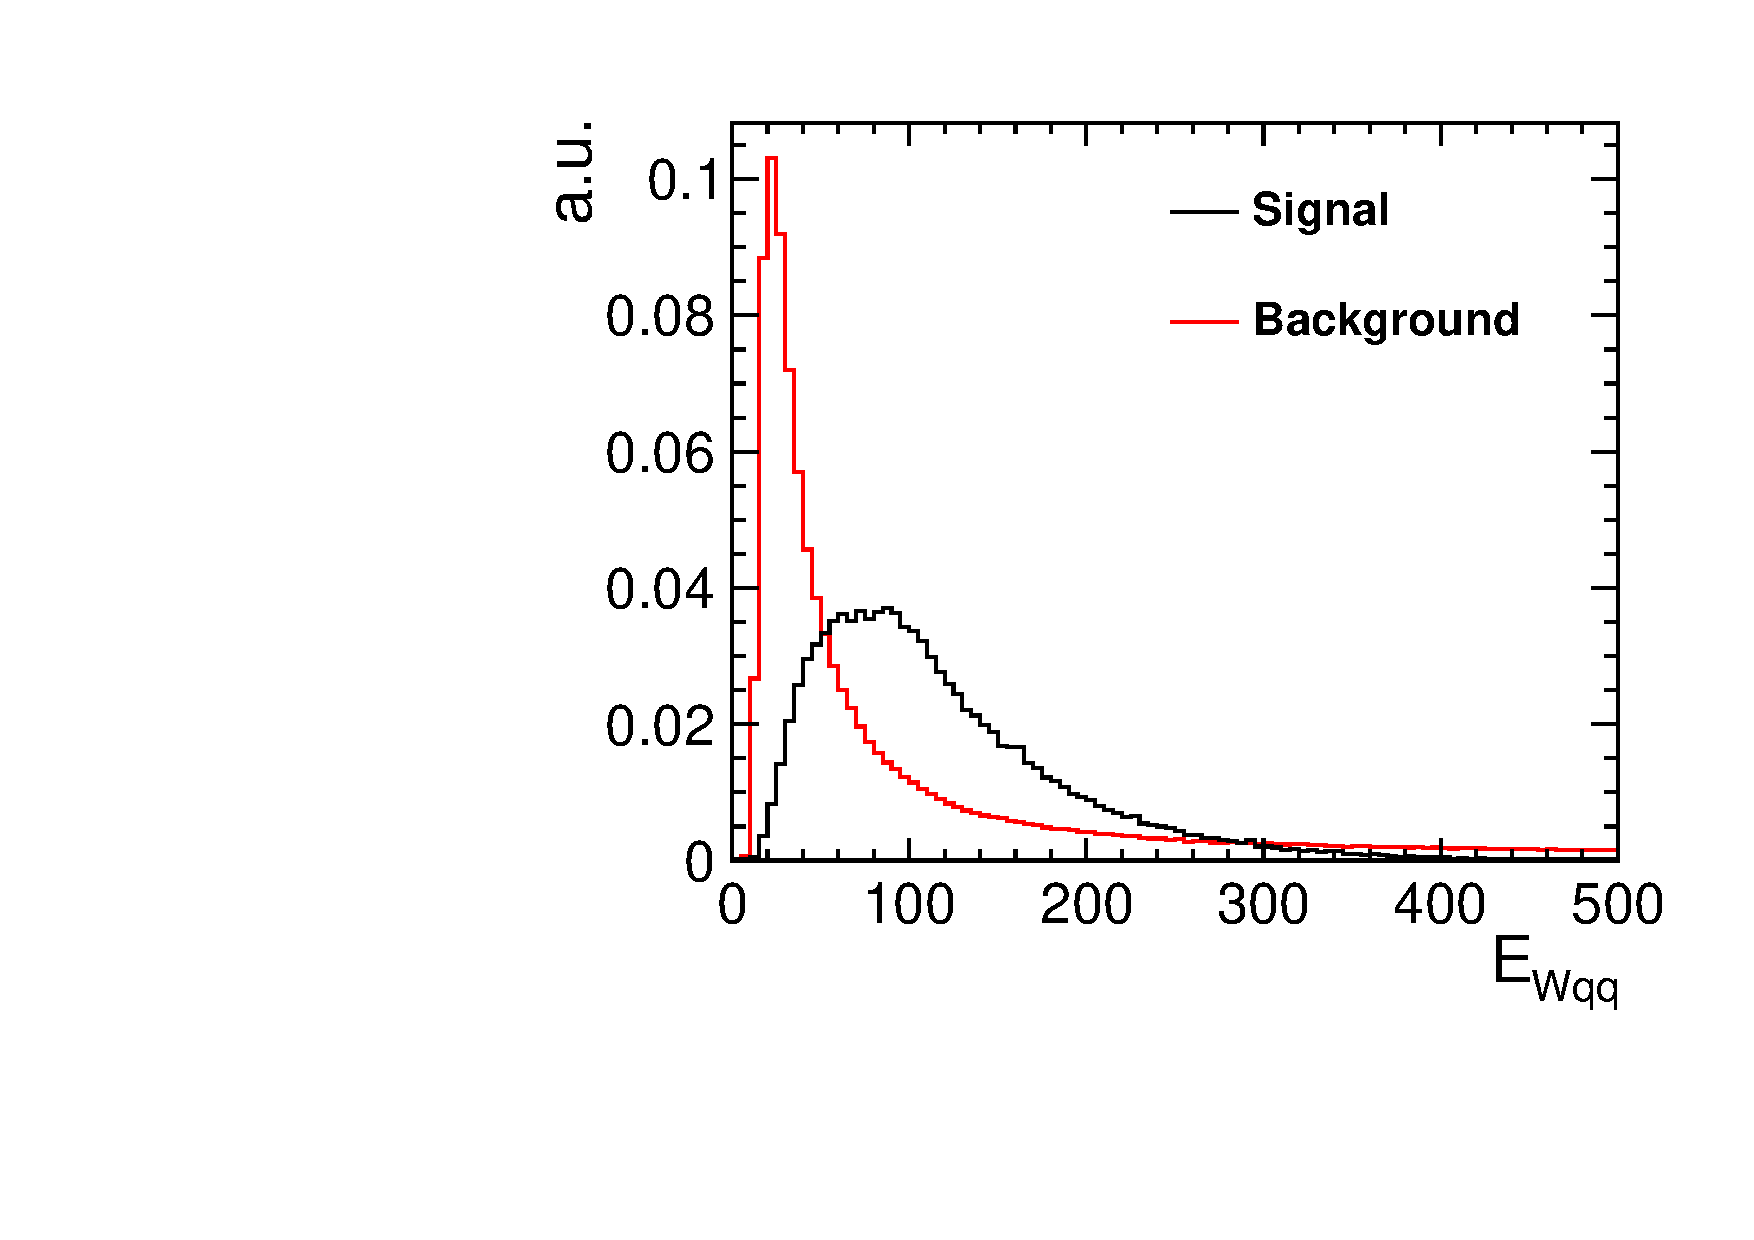
\includegraphics[width=0.75\linewidth]{Appendix/figures/EWqq} 
    \caption{Energy of hadronically decaying W} 
    \vspace{4ex}
  \end{subfigure}%% 
  \begin{subfigure}[]{0.5\linewidth}
    \centering
    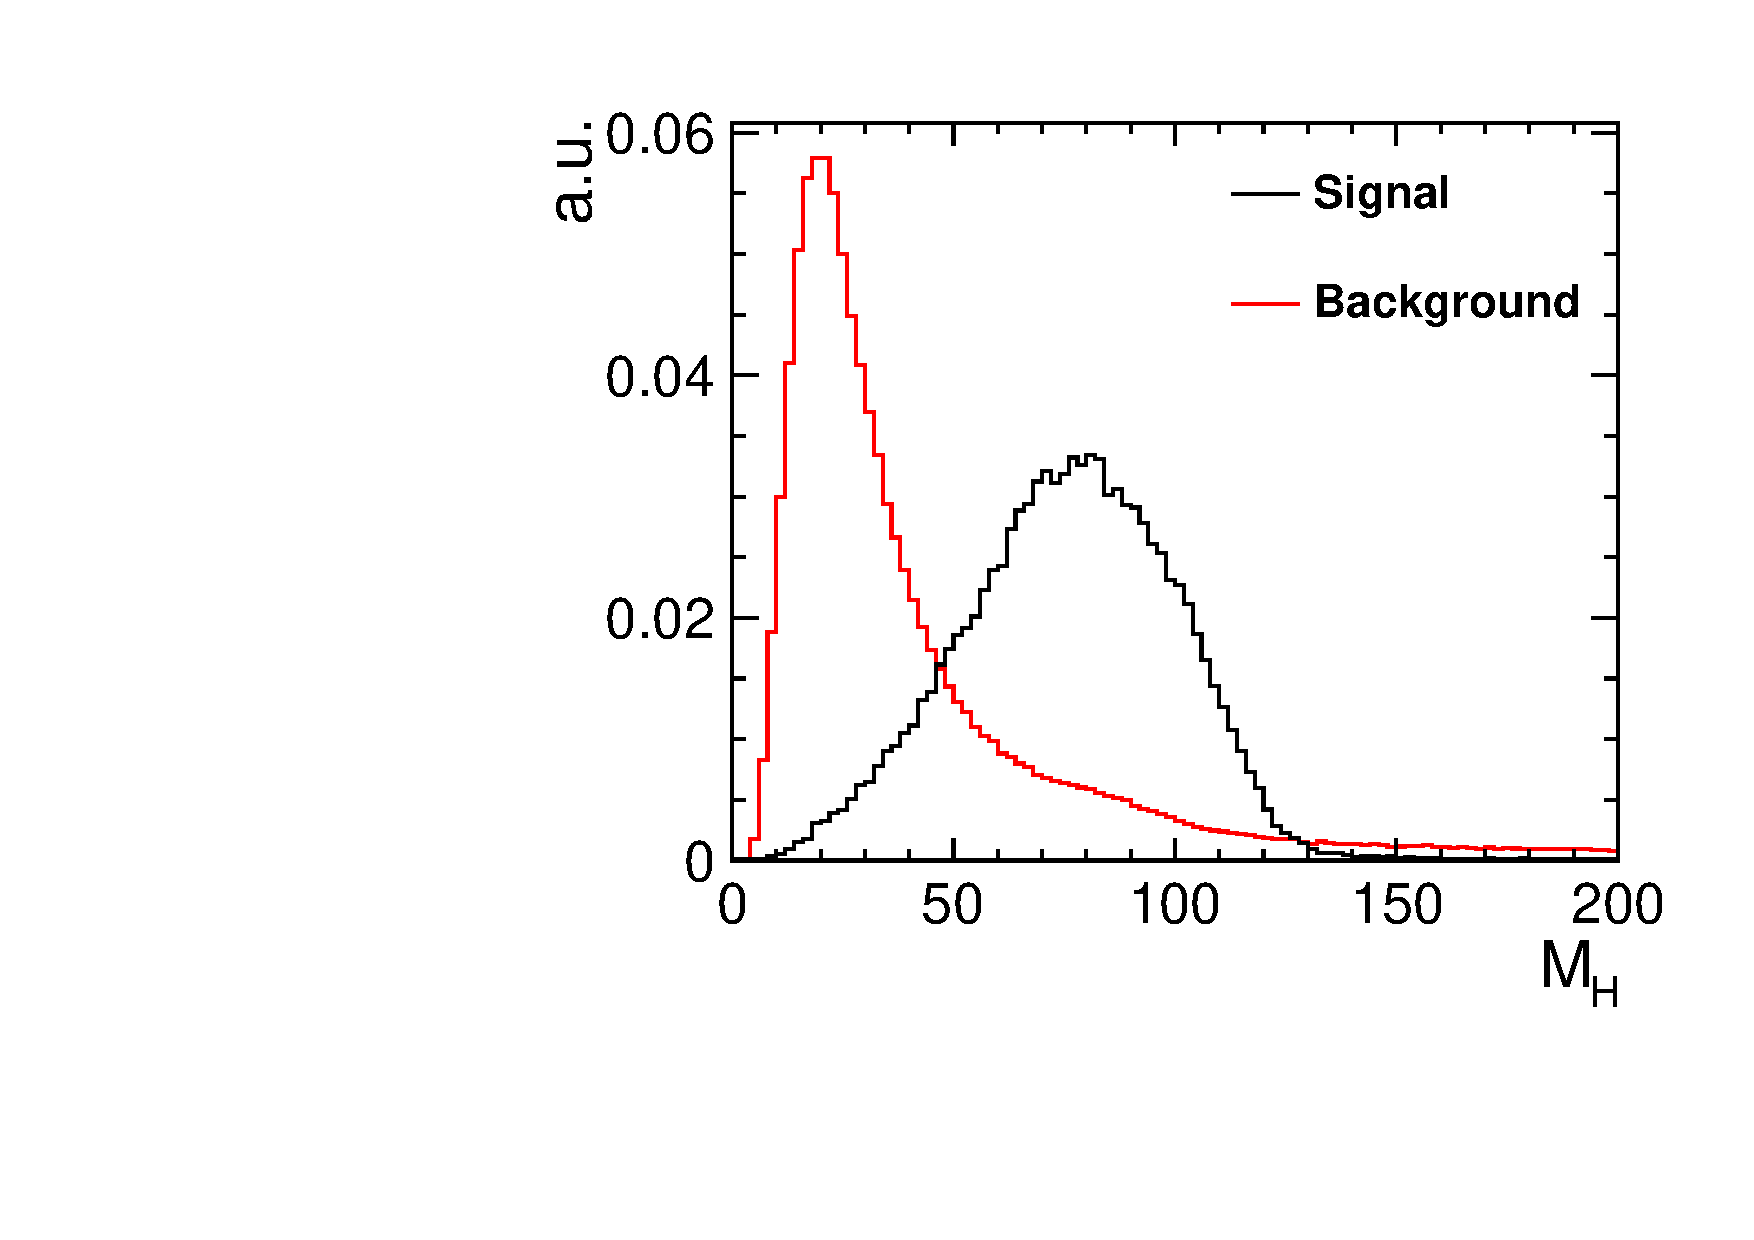
\includegraphics[width=0.75\linewidth]{Appendix/figures/HiggsMass} 
    \caption{Reconstructed Higgs mass} 
    \vspace{4ex}
  \end{subfigure}
    \begin{subfigure}[]{0.5\linewidth}
    \centering
    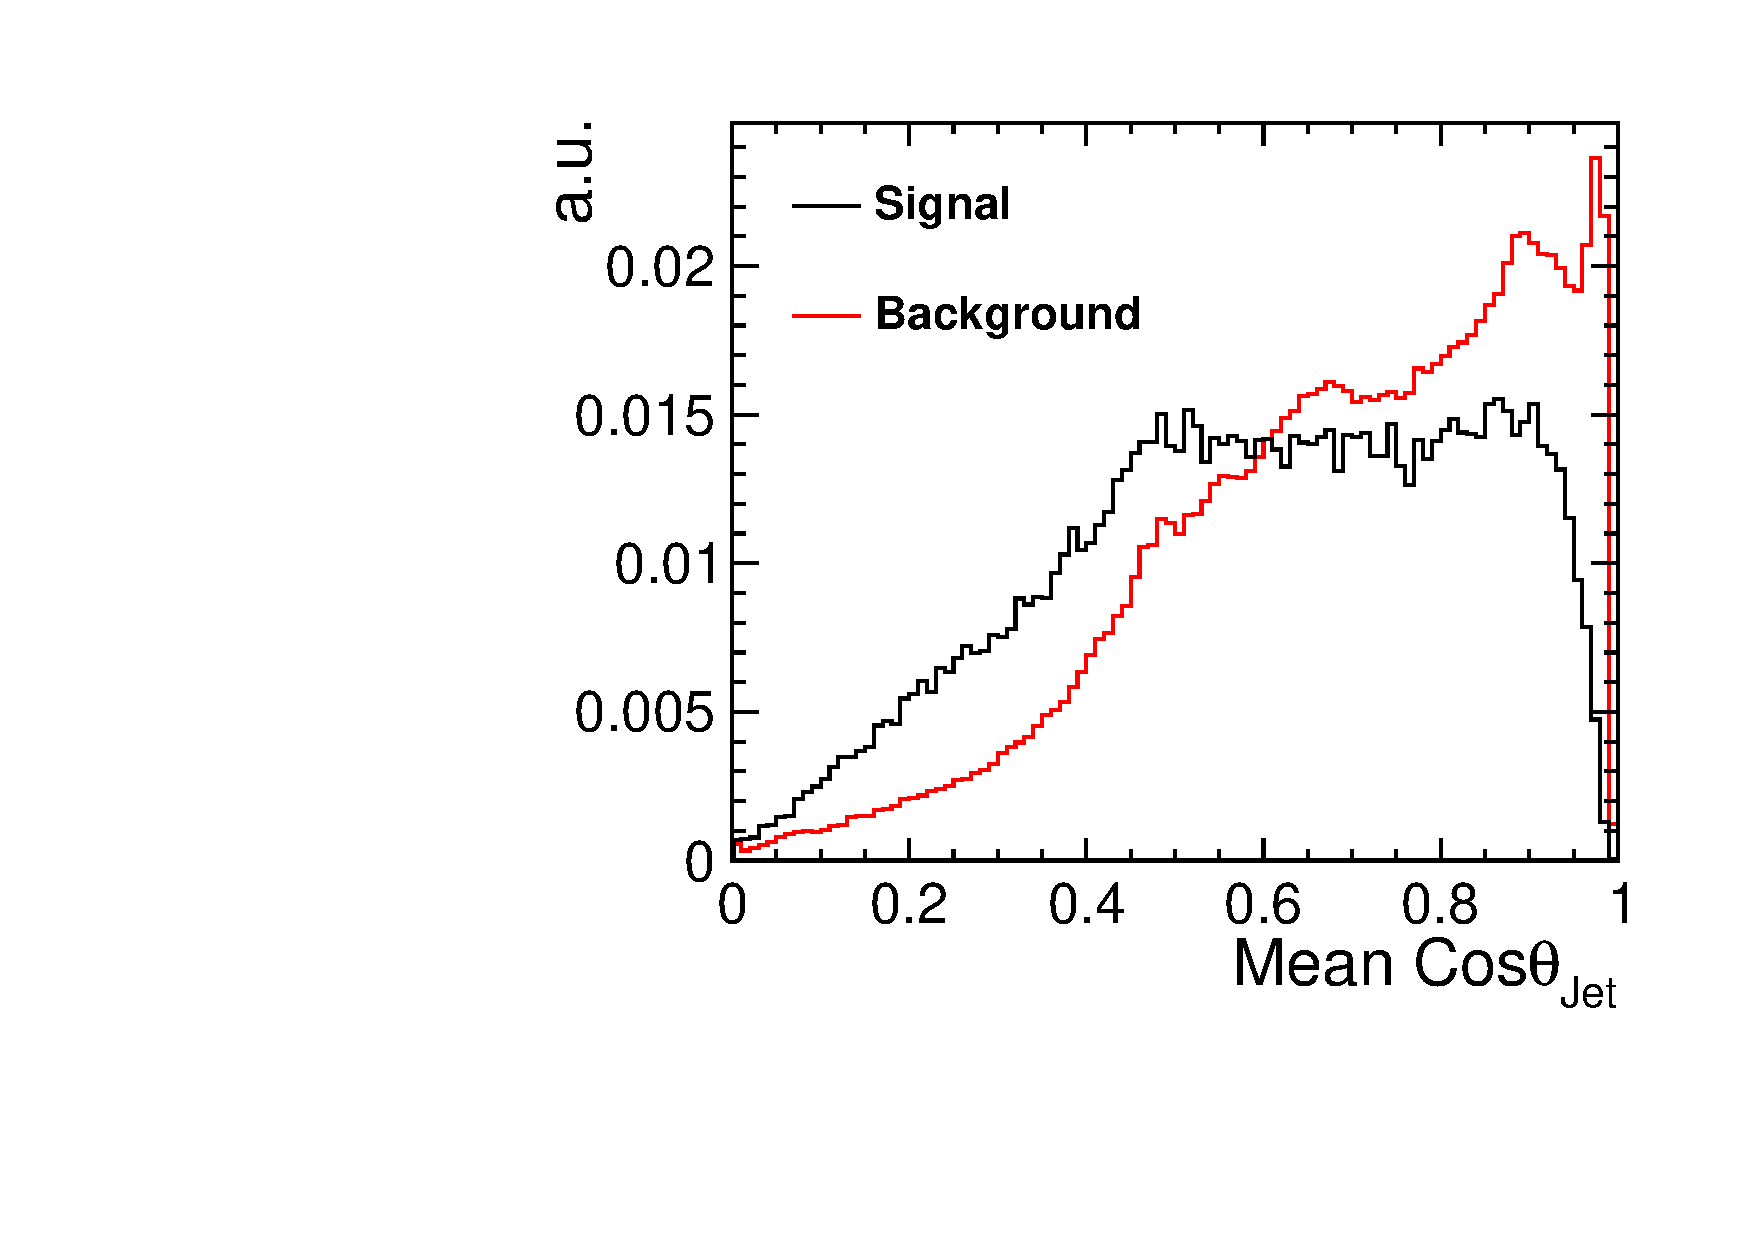
\includegraphics[width=0.75\linewidth]{Appendix/figures/JetCosTheta} 
    \caption{Average cos$\theta$ of jets} 
  \end{subfigure}%%
  \begin{subfigure}[]{0.5\linewidth}
    \centering
    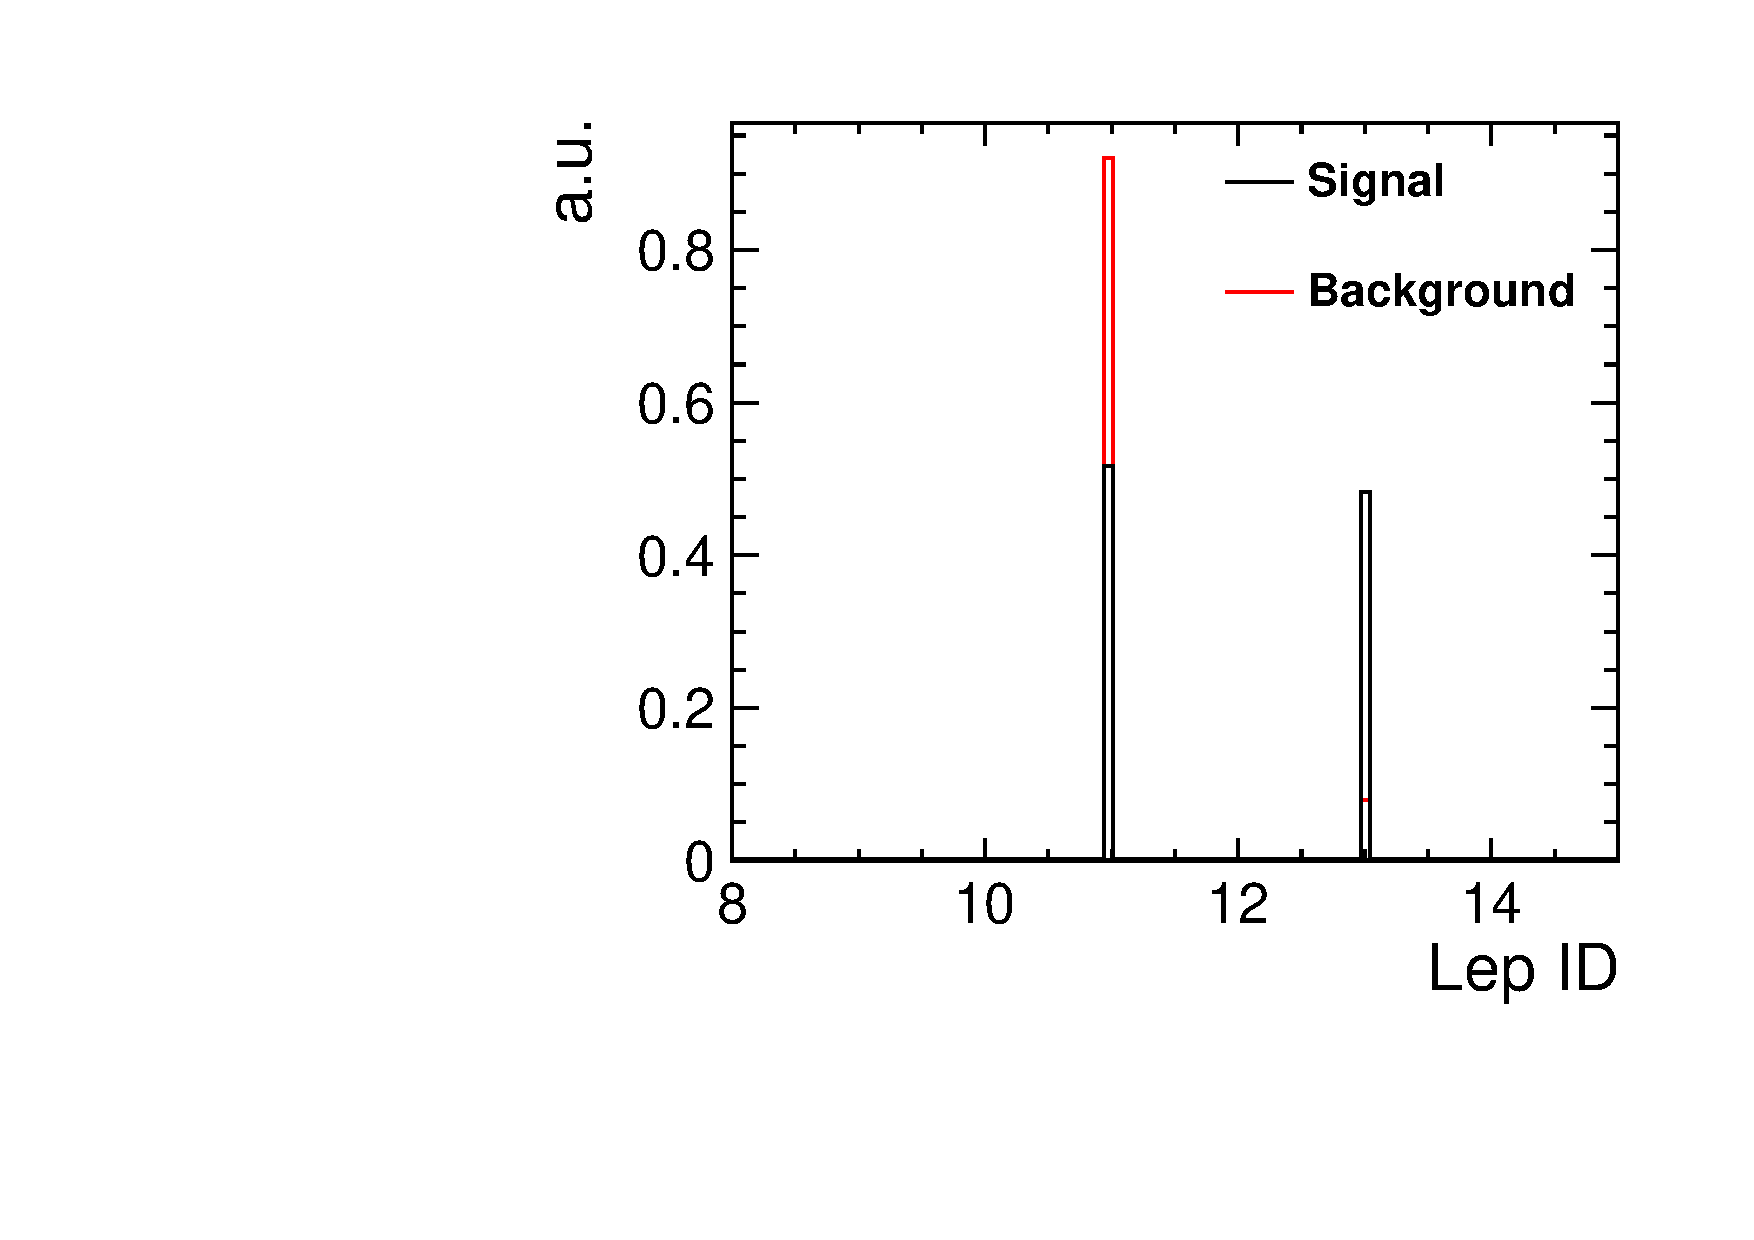
\includegraphics[width=0.75\linewidth]{Appendix/figures/LepID} 
    \caption{Lepton PID} 
  \end{subfigure}
\end{figure}


\begin{figure}[]\ContinuedFloat
    \begin{subfigure}[]{0.5\linewidth}
    \centering
    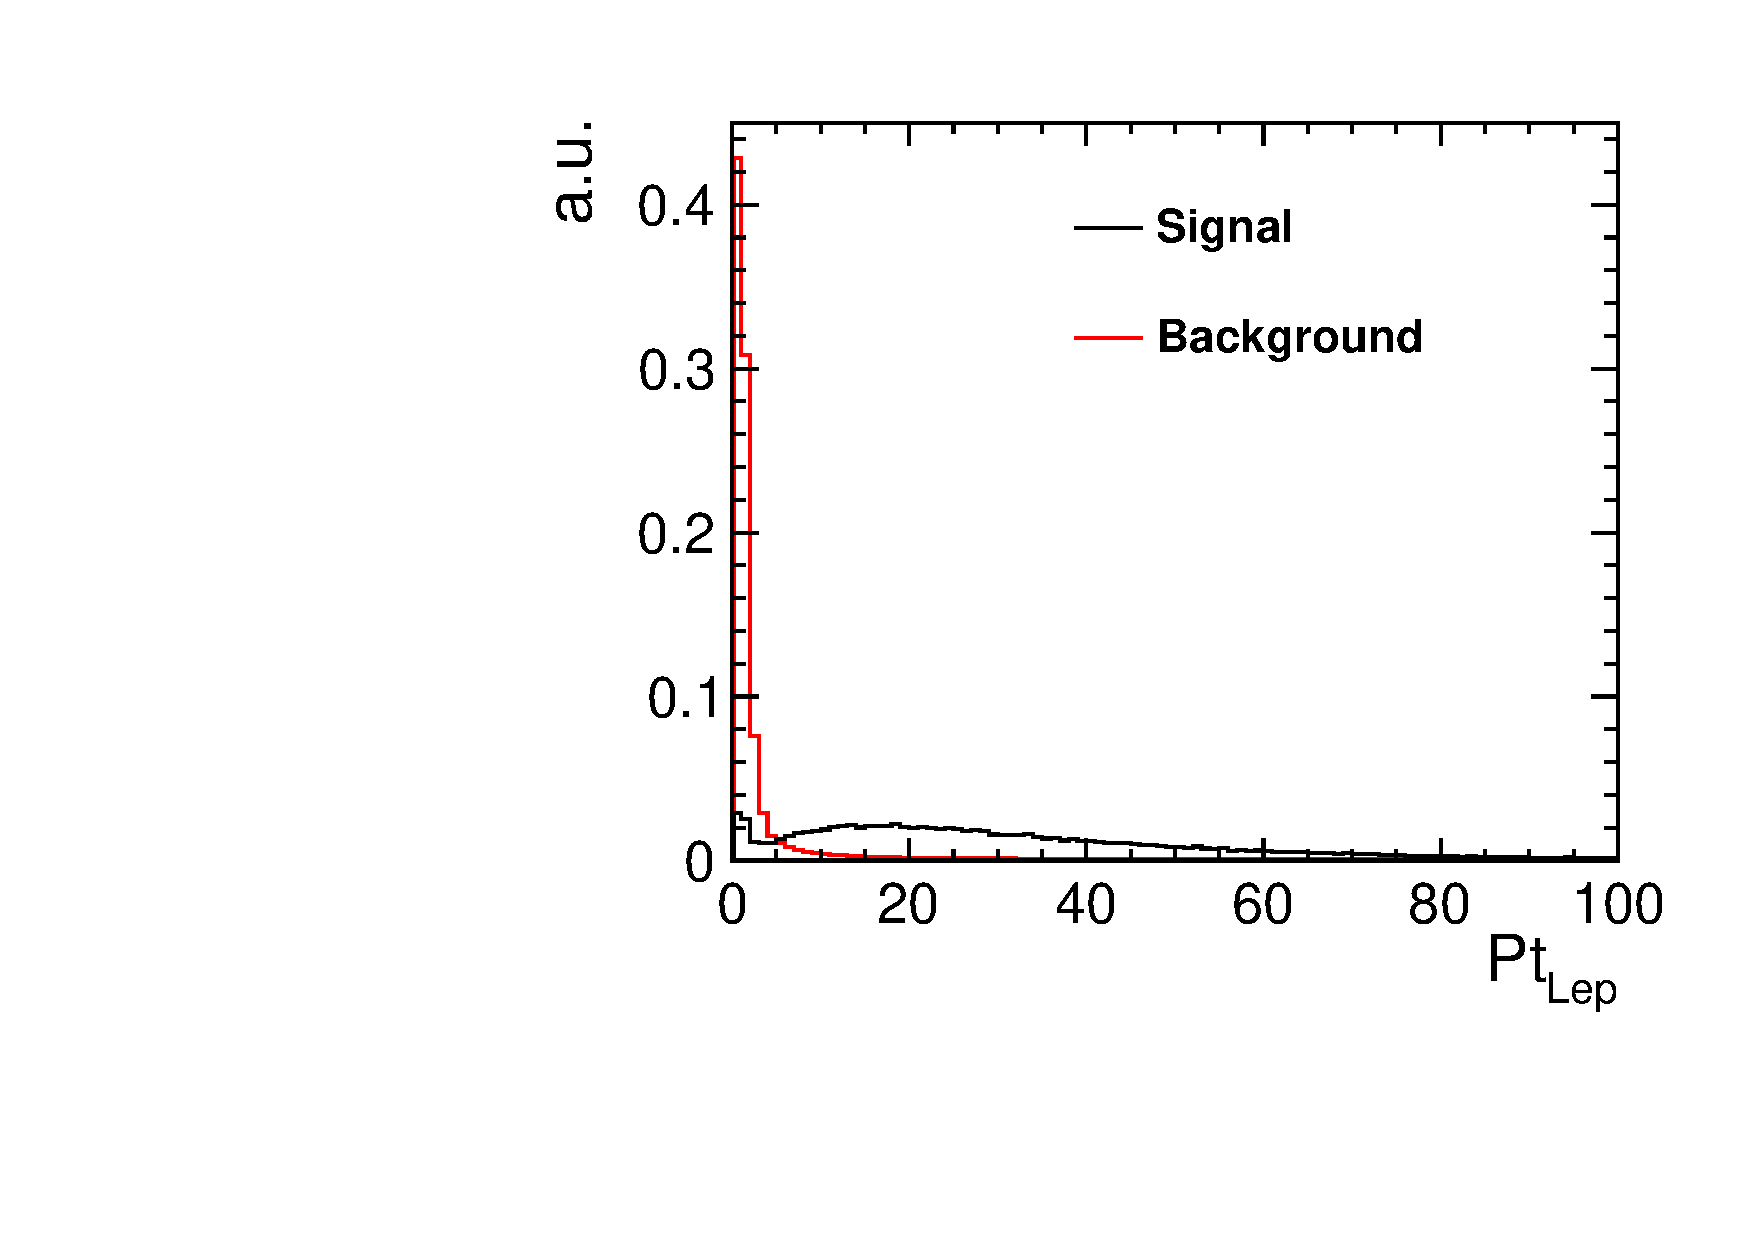
\includegraphics[width=0.75\linewidth]{Appendix/figures/LepPt} 
    \caption{Lepton Pt} 
  \end{subfigure}%%
  \begin{subfigure}[]{0.5\linewidth}
    \centering
    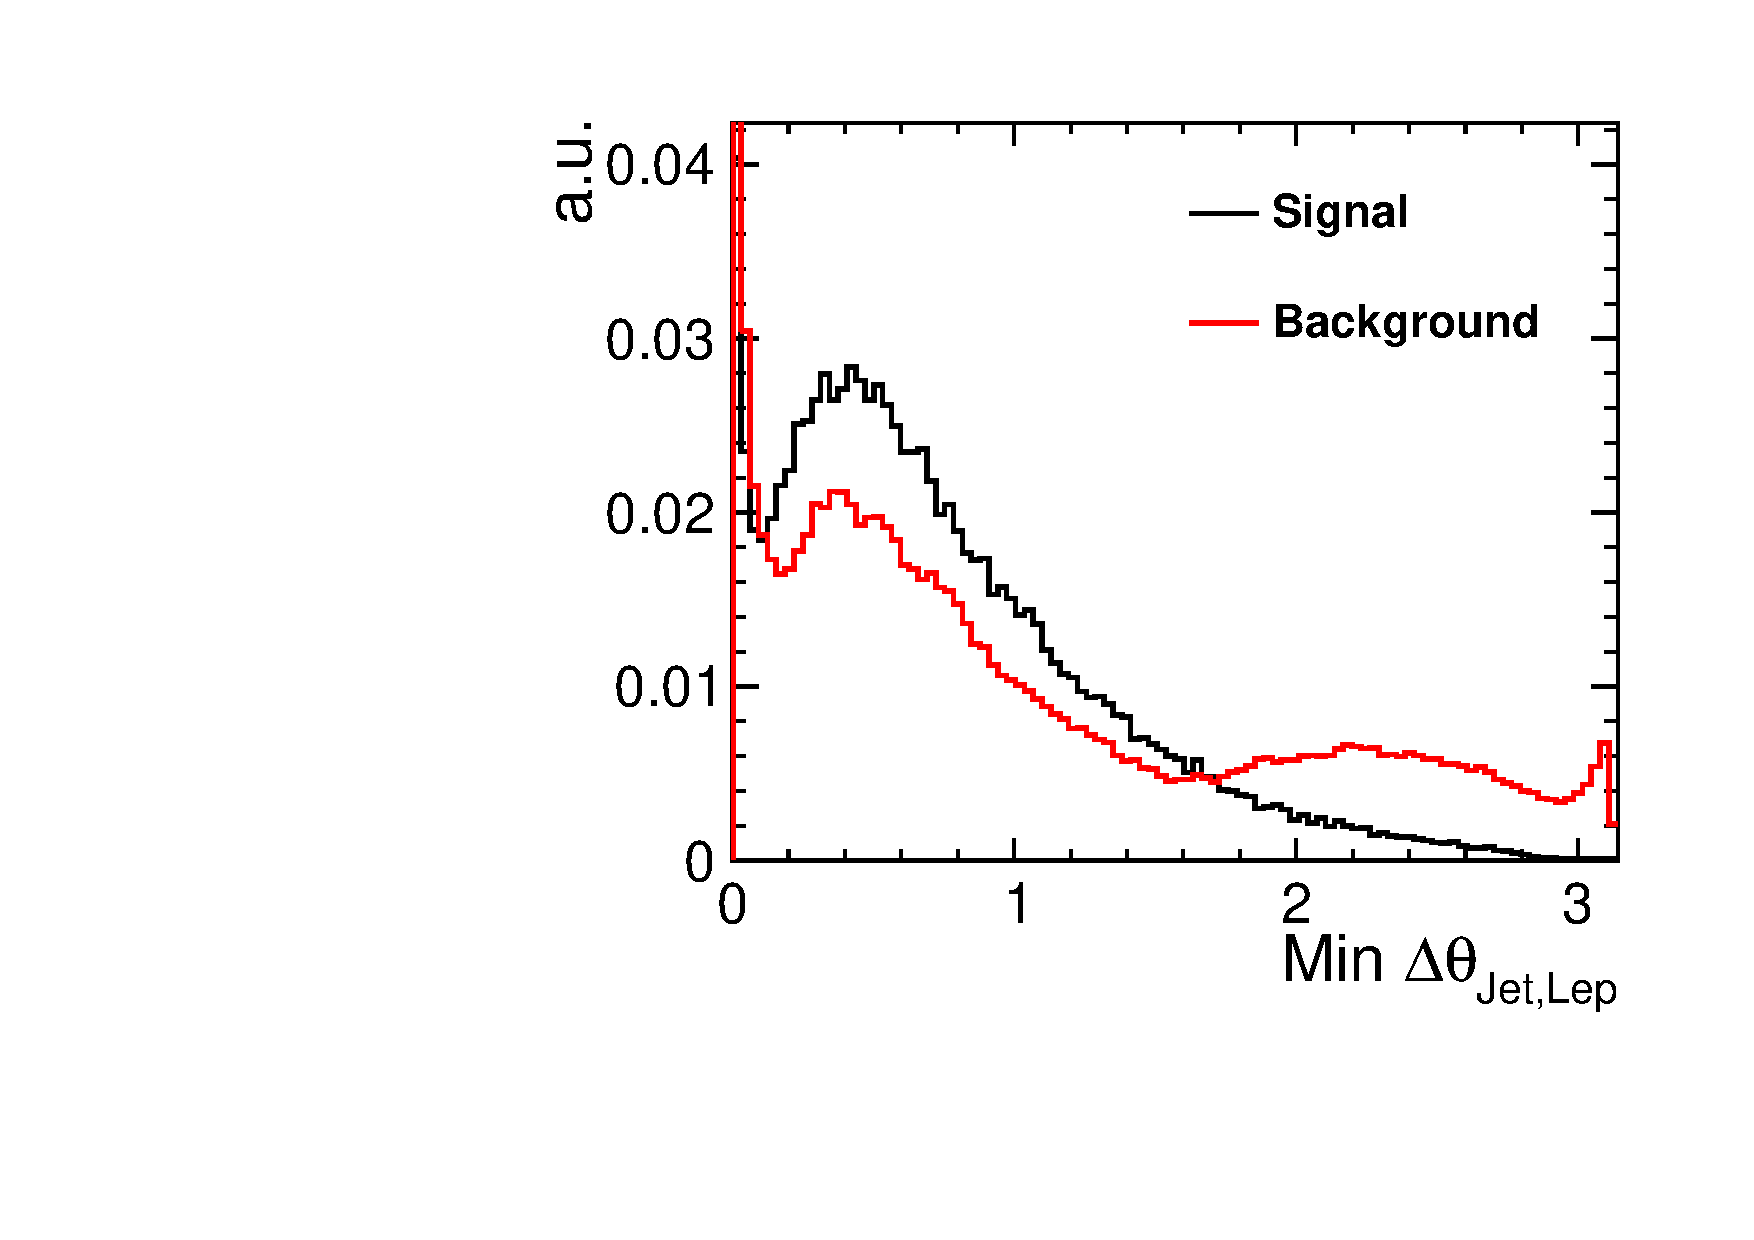
\includegraphics[width=0.75\linewidth]{Appendix/figures/MinJetLepAngSep} 
    \caption{Angular separation between lepton and nearest jet} 
  \end{subfigure}
  \begin{subfigure}[]{0.5\linewidth}
    \centering
    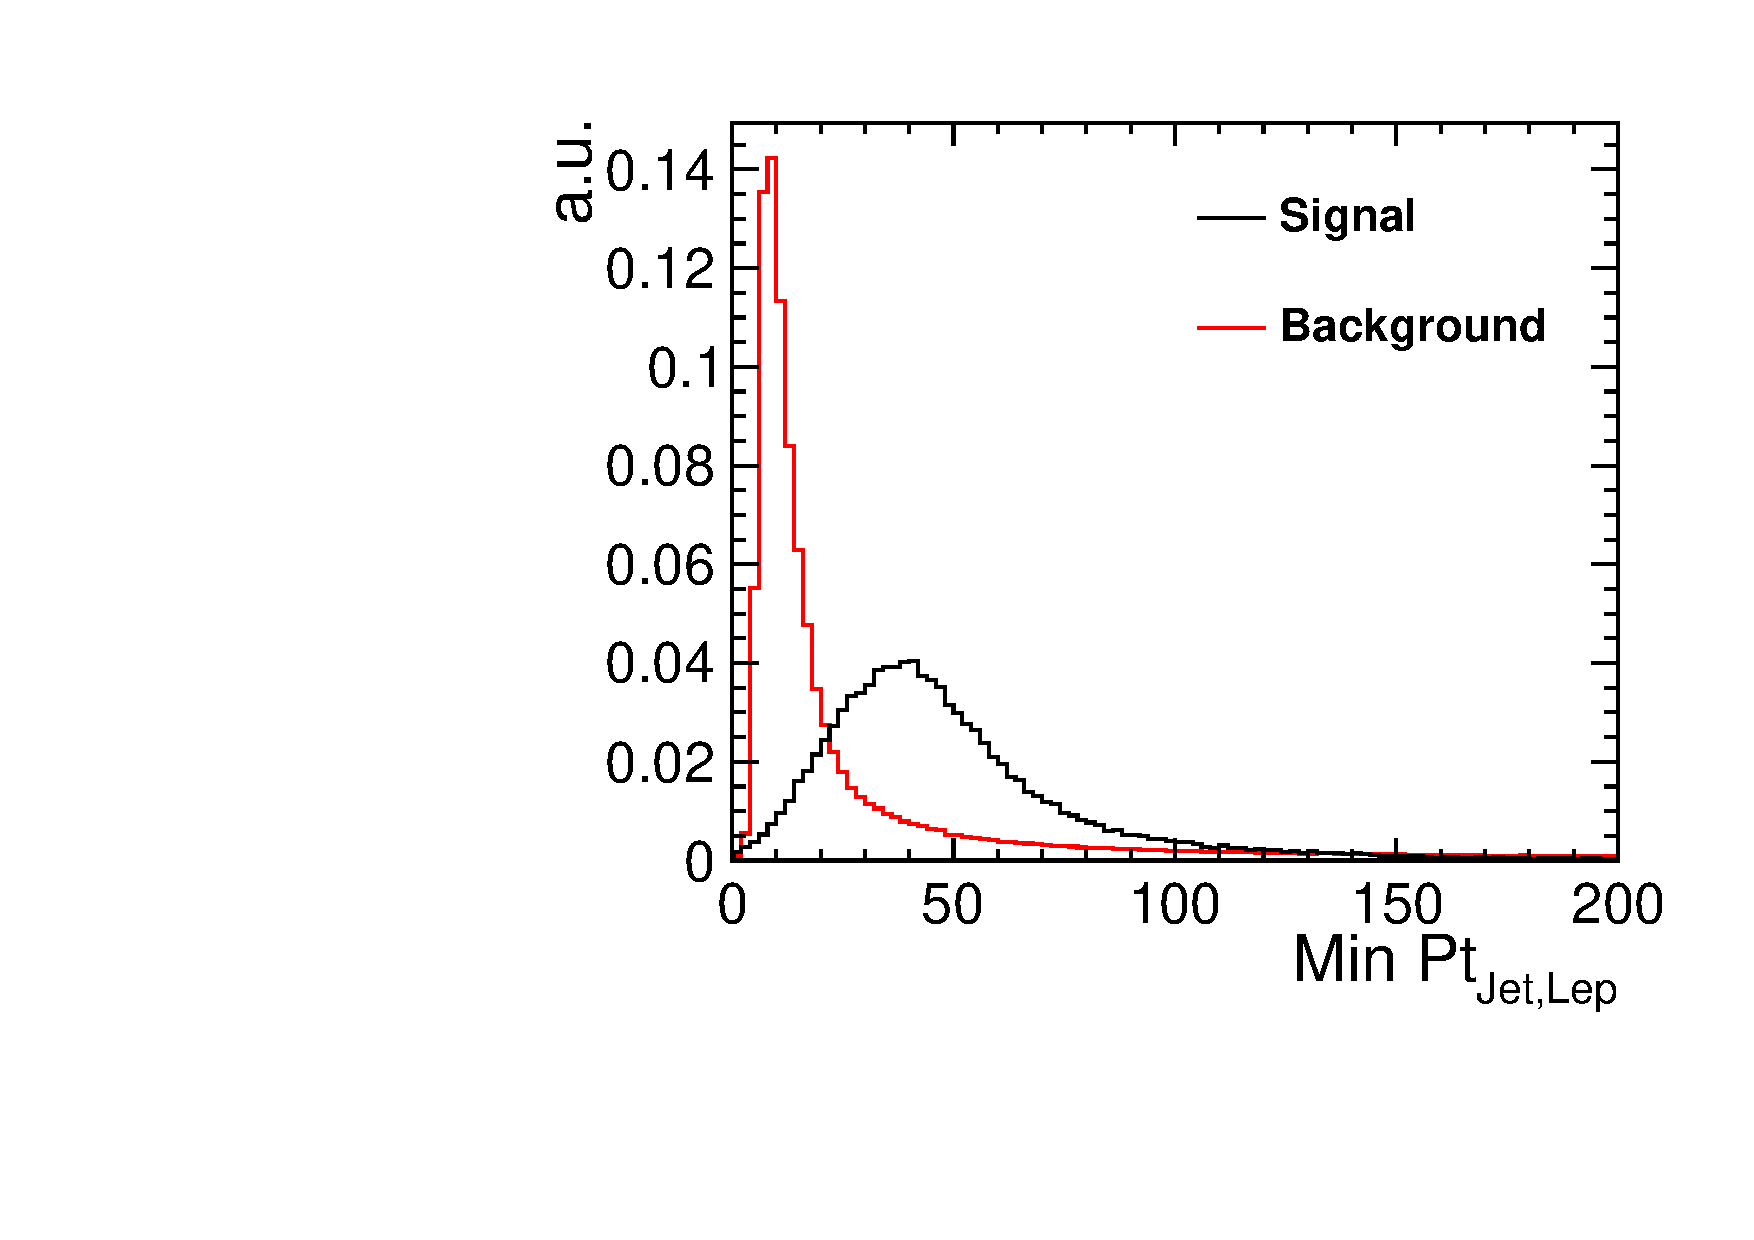
\includegraphics[width=0.75\linewidth]{Appendix/figures/MinJetLepPt} 
    \caption{Relative Pt between lepton and nearest jet} 
    \vspace{4ex}
  \end{subfigure}%% 
  \begin{subfigure}[]{0.5\linewidth}
    \centering
    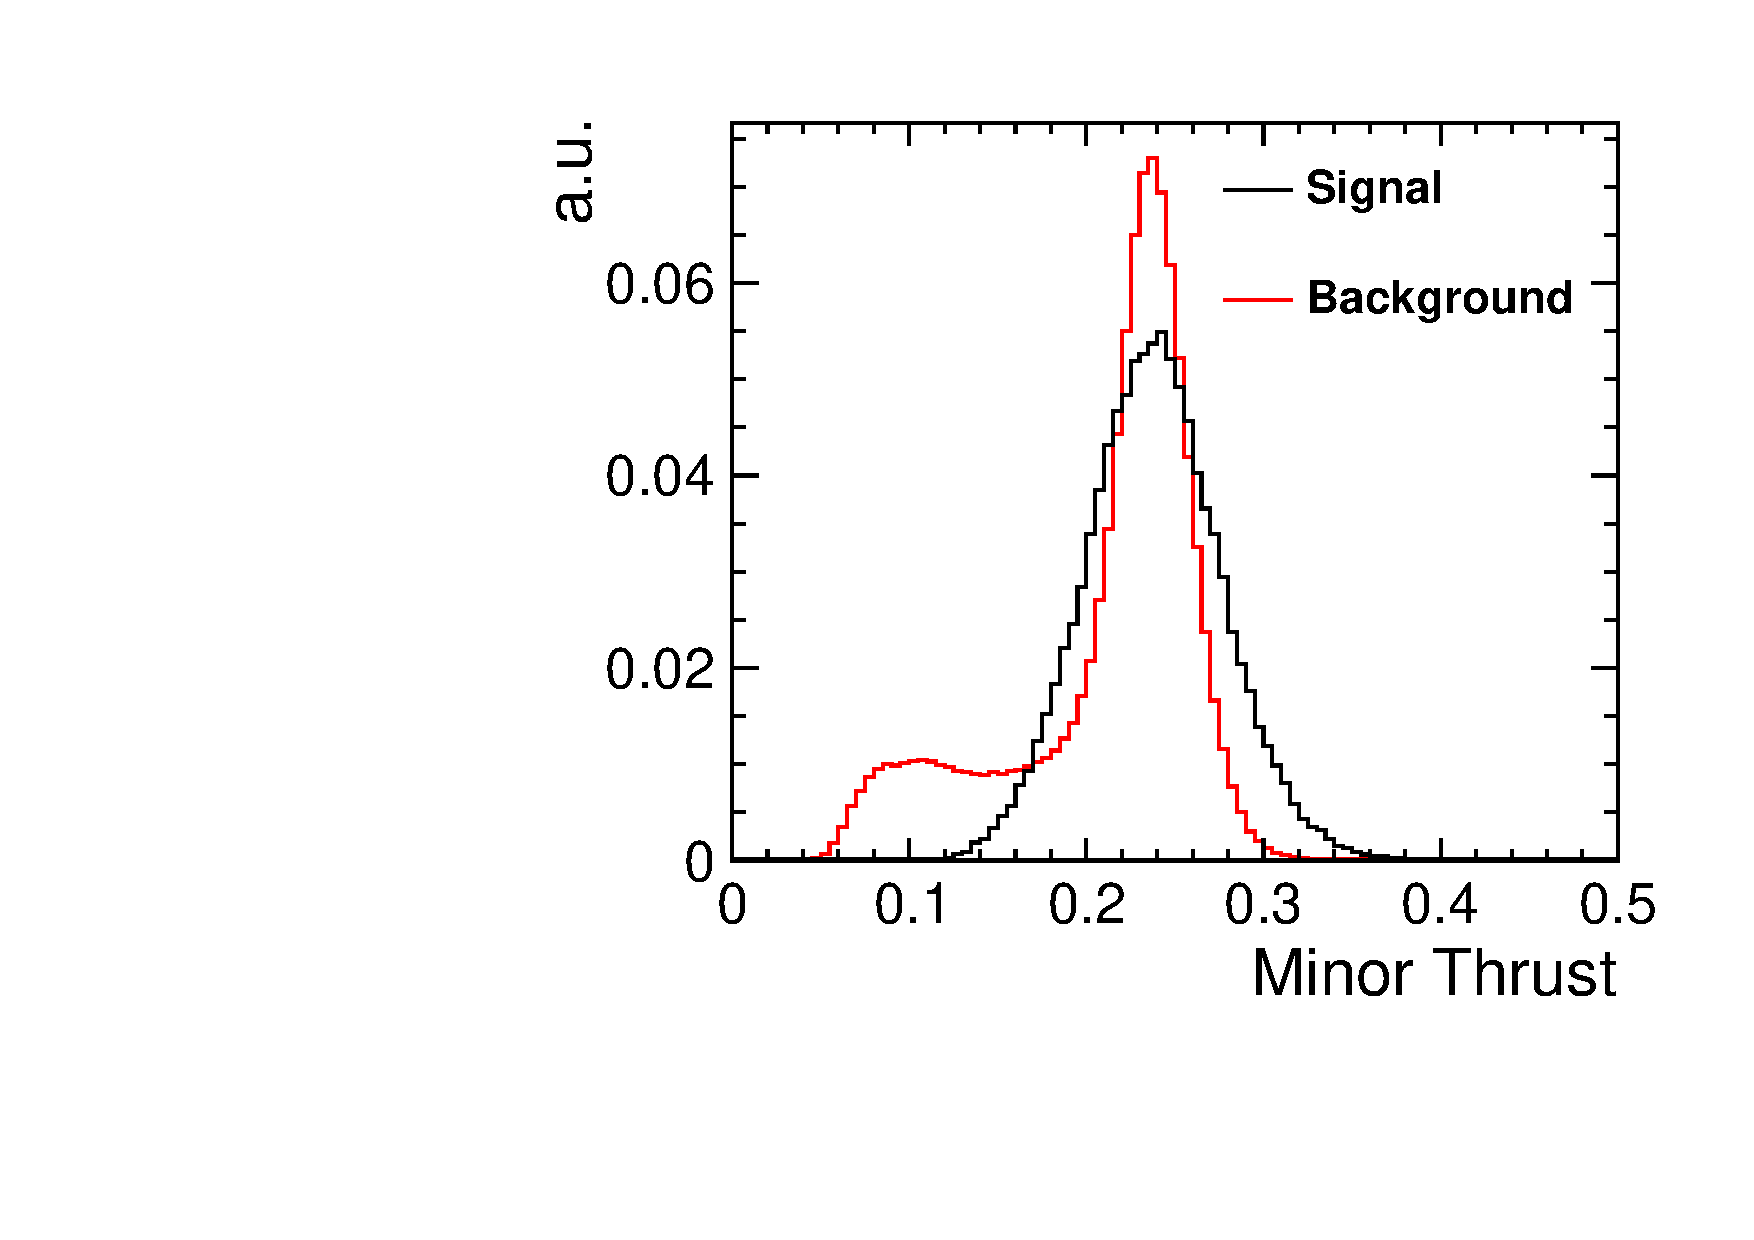
\includegraphics[width=0.75\linewidth]{Appendix/figures/MinorThrust} 
    \caption{Minor Thrust of the event} 
    \vspace{4ex}
  \end{subfigure} 
  \begin{subfigure}[]{0.5\linewidth}
    \centering
    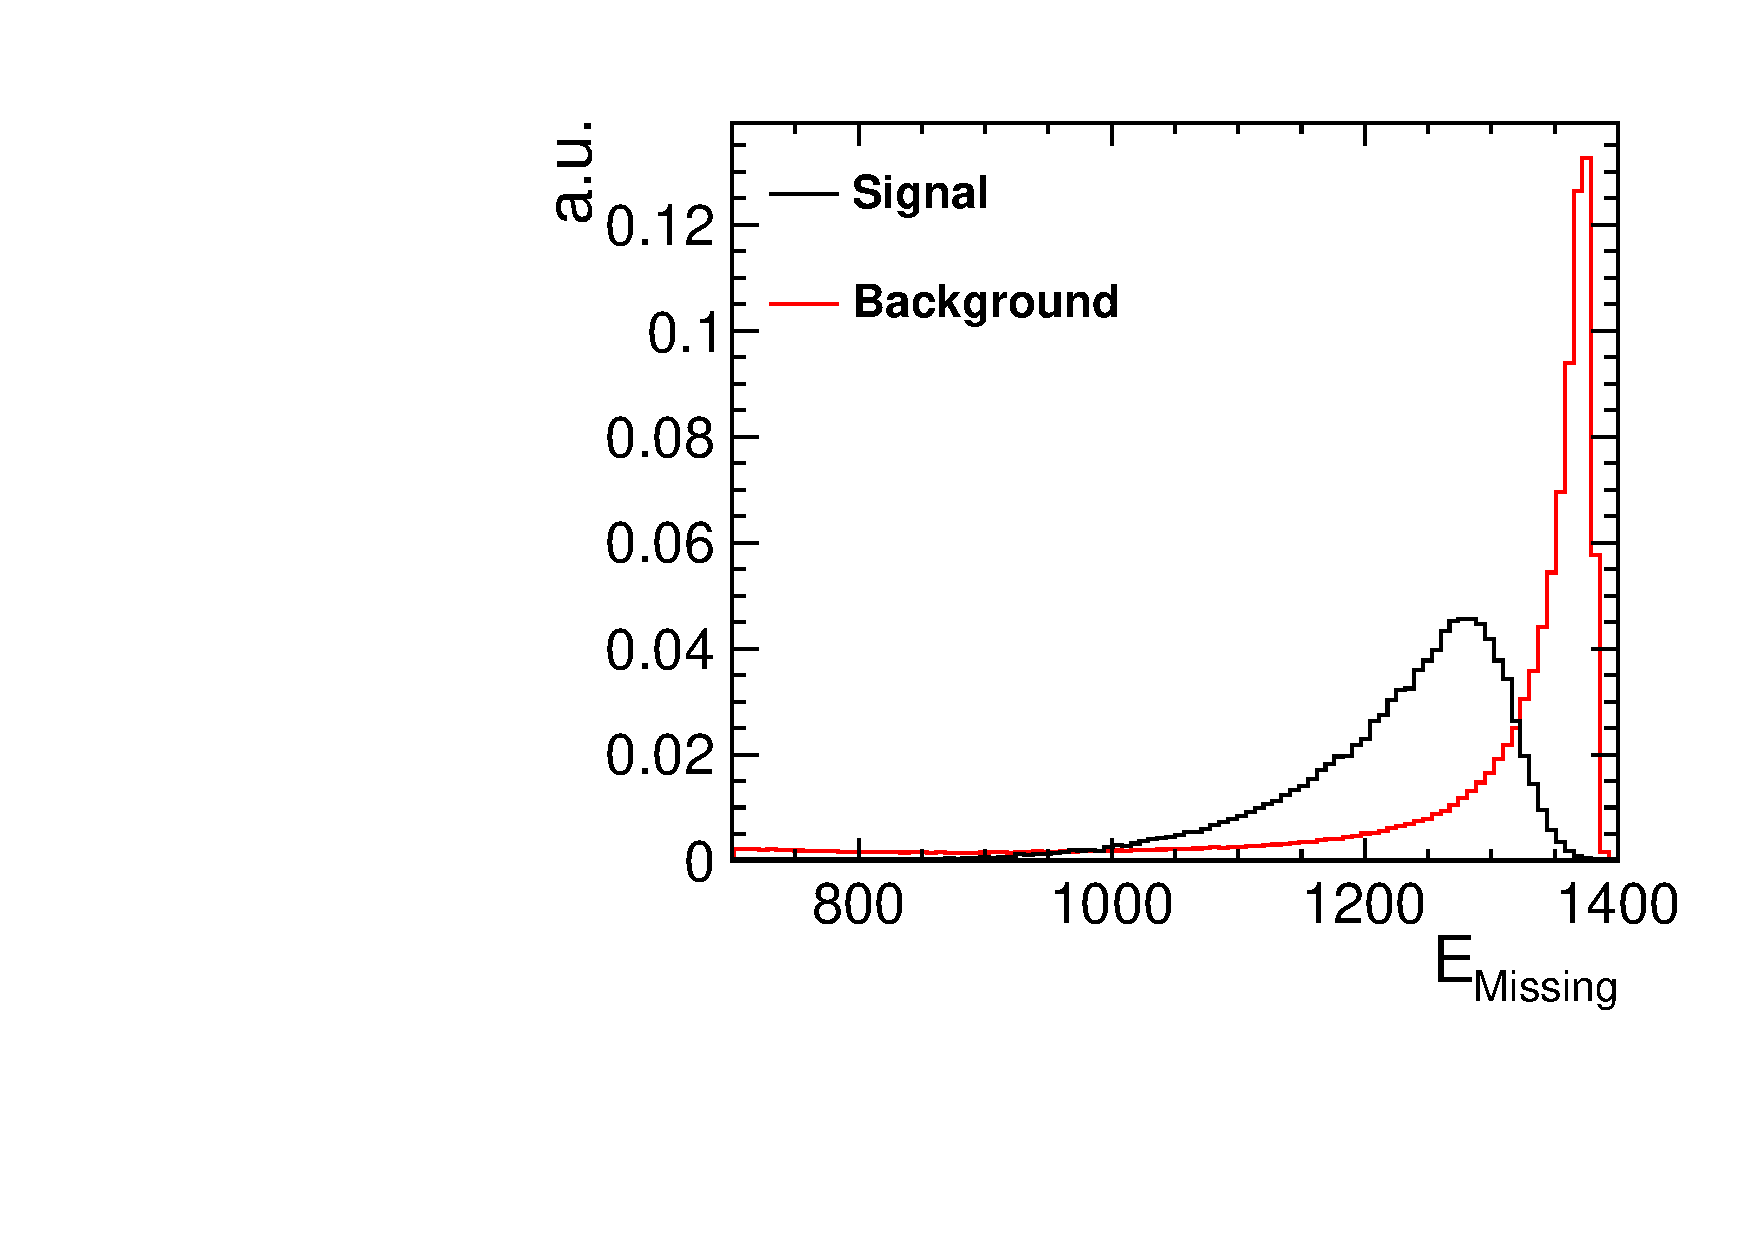
\includegraphics[width=0.75\linewidth]{Appendix/figures/MissingE} 
    \caption{Missing energy} 
    \vspace{4ex}
  \end{subfigure}%%
  \begin{subfigure}[]{0.5\linewidth}
    \centering
    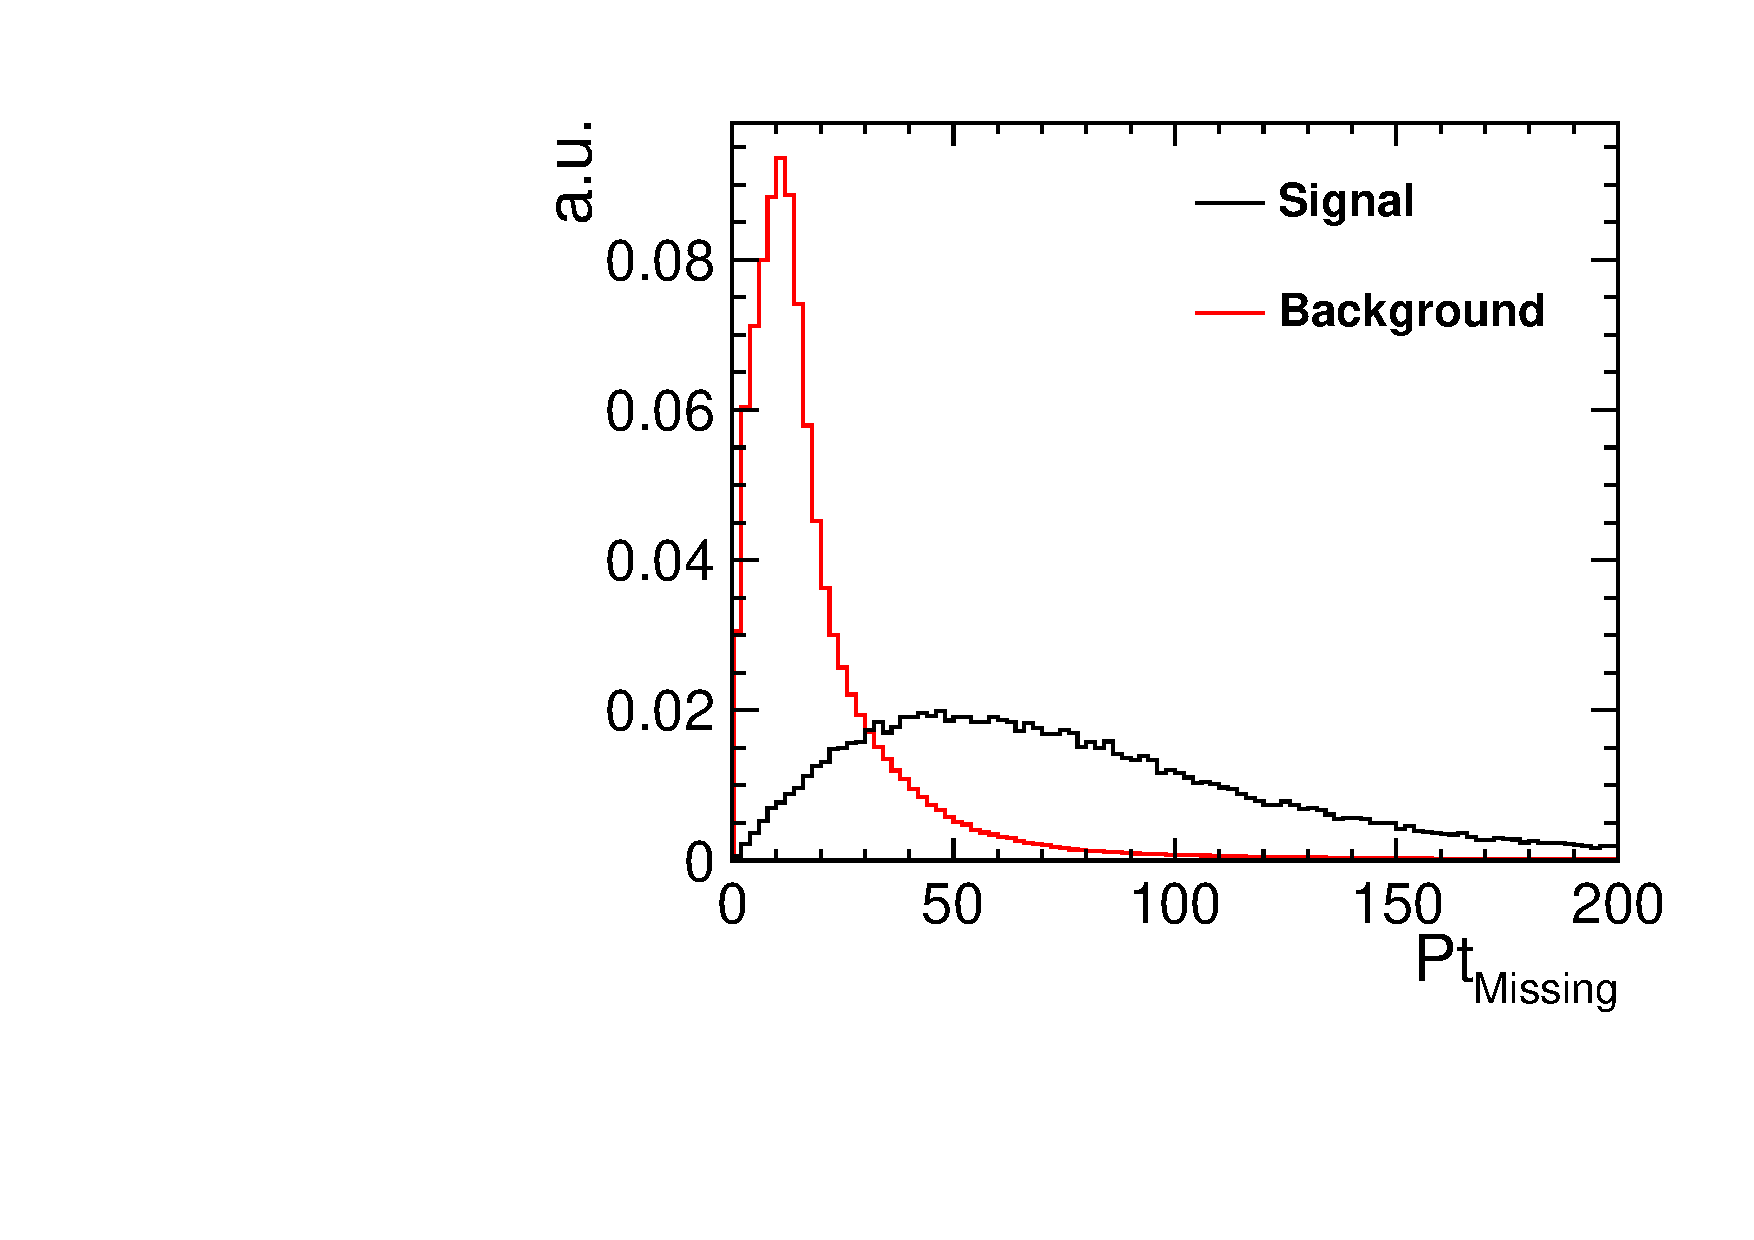
\includegraphics[width=0.75\linewidth]{Appendix/figures/MissingPt} 
    \caption{Missing transverse momentum} 
    \vspace{4ex}
  \end{subfigure}
\end{figure}

\begin{figure}[]\ContinuedFloat 
   \begin{subfigure}[]{0.5\linewidth}
    \centering
    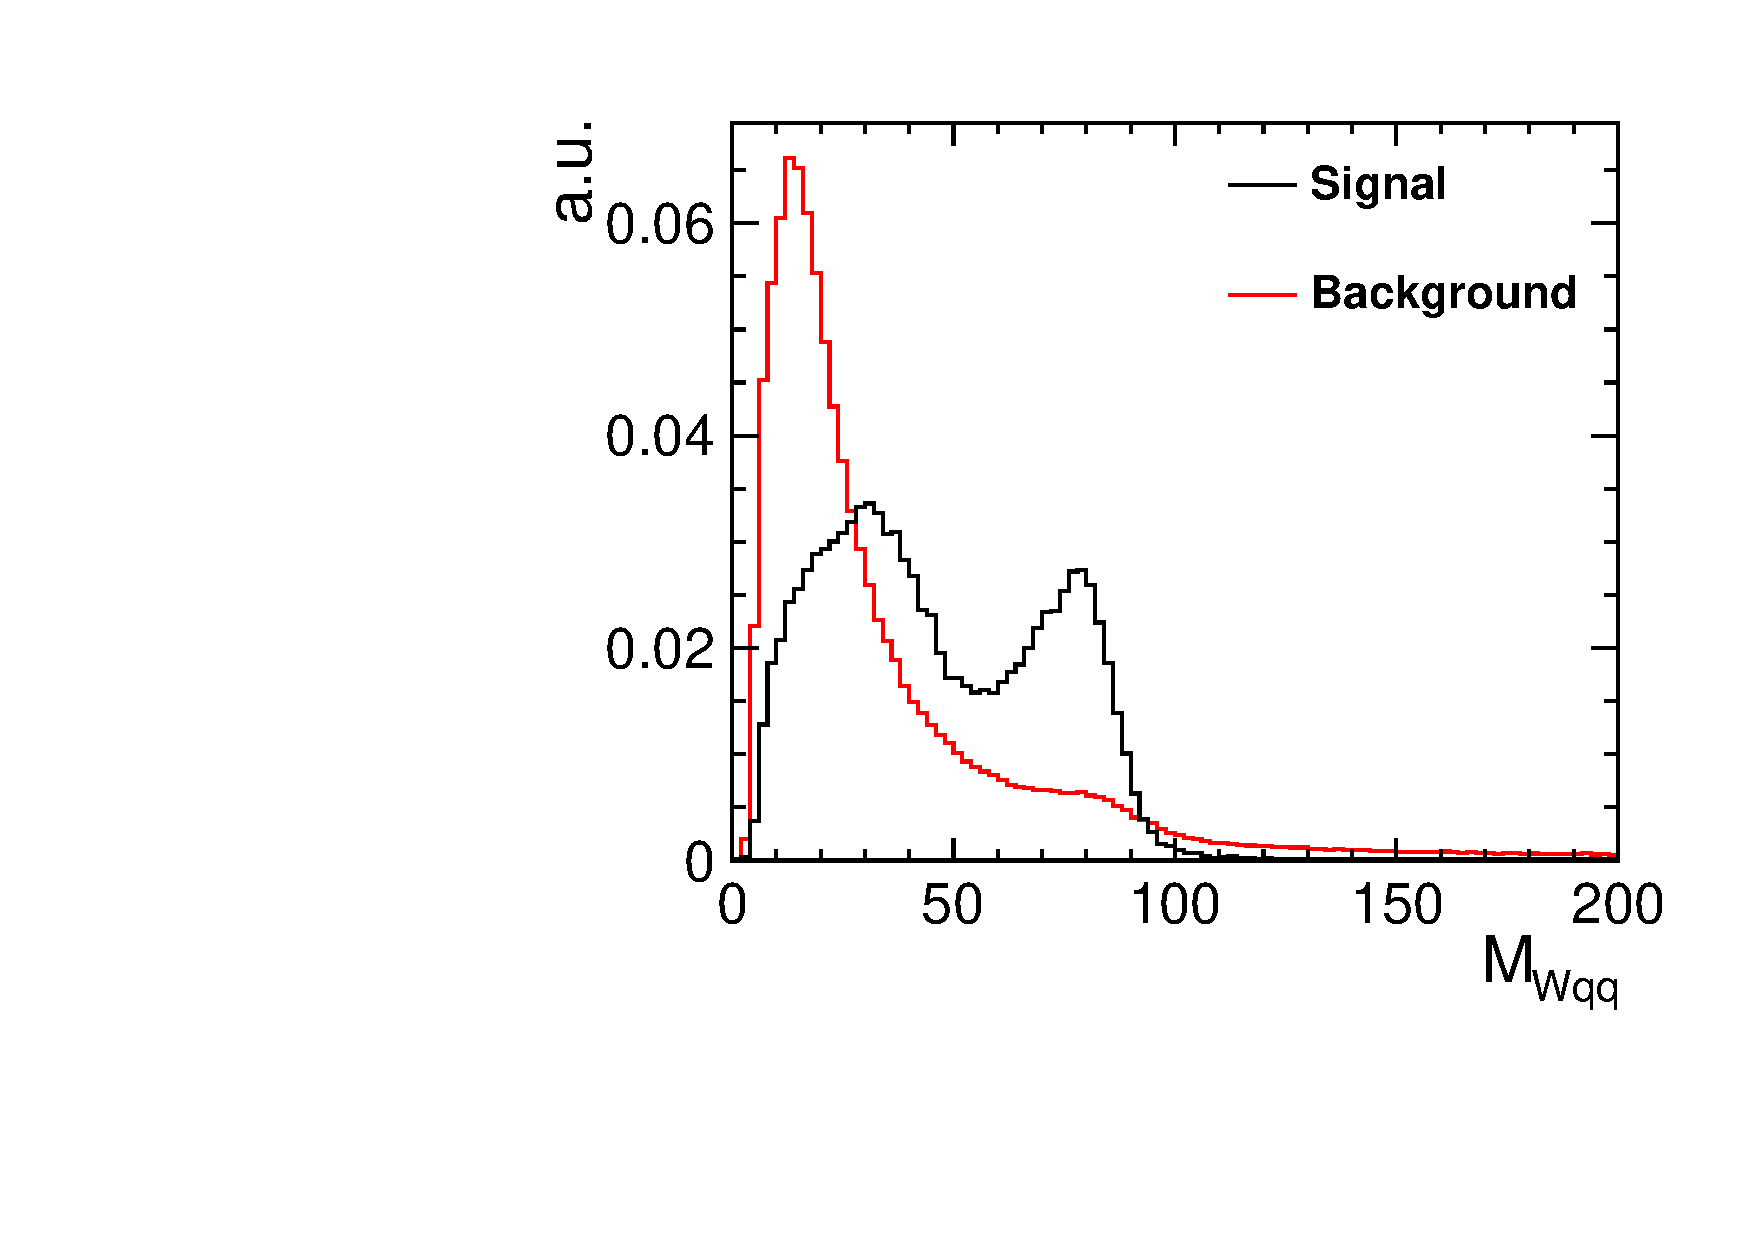
\includegraphics[width=0.75\linewidth]{Appendix/figures/MWqq} 
    \caption{Mass of hadronically decaying W} 
    \vspace{4ex}
  \end{subfigure}%%
  \begin{subfigure}[]{0.5\linewidth}
    \centering
    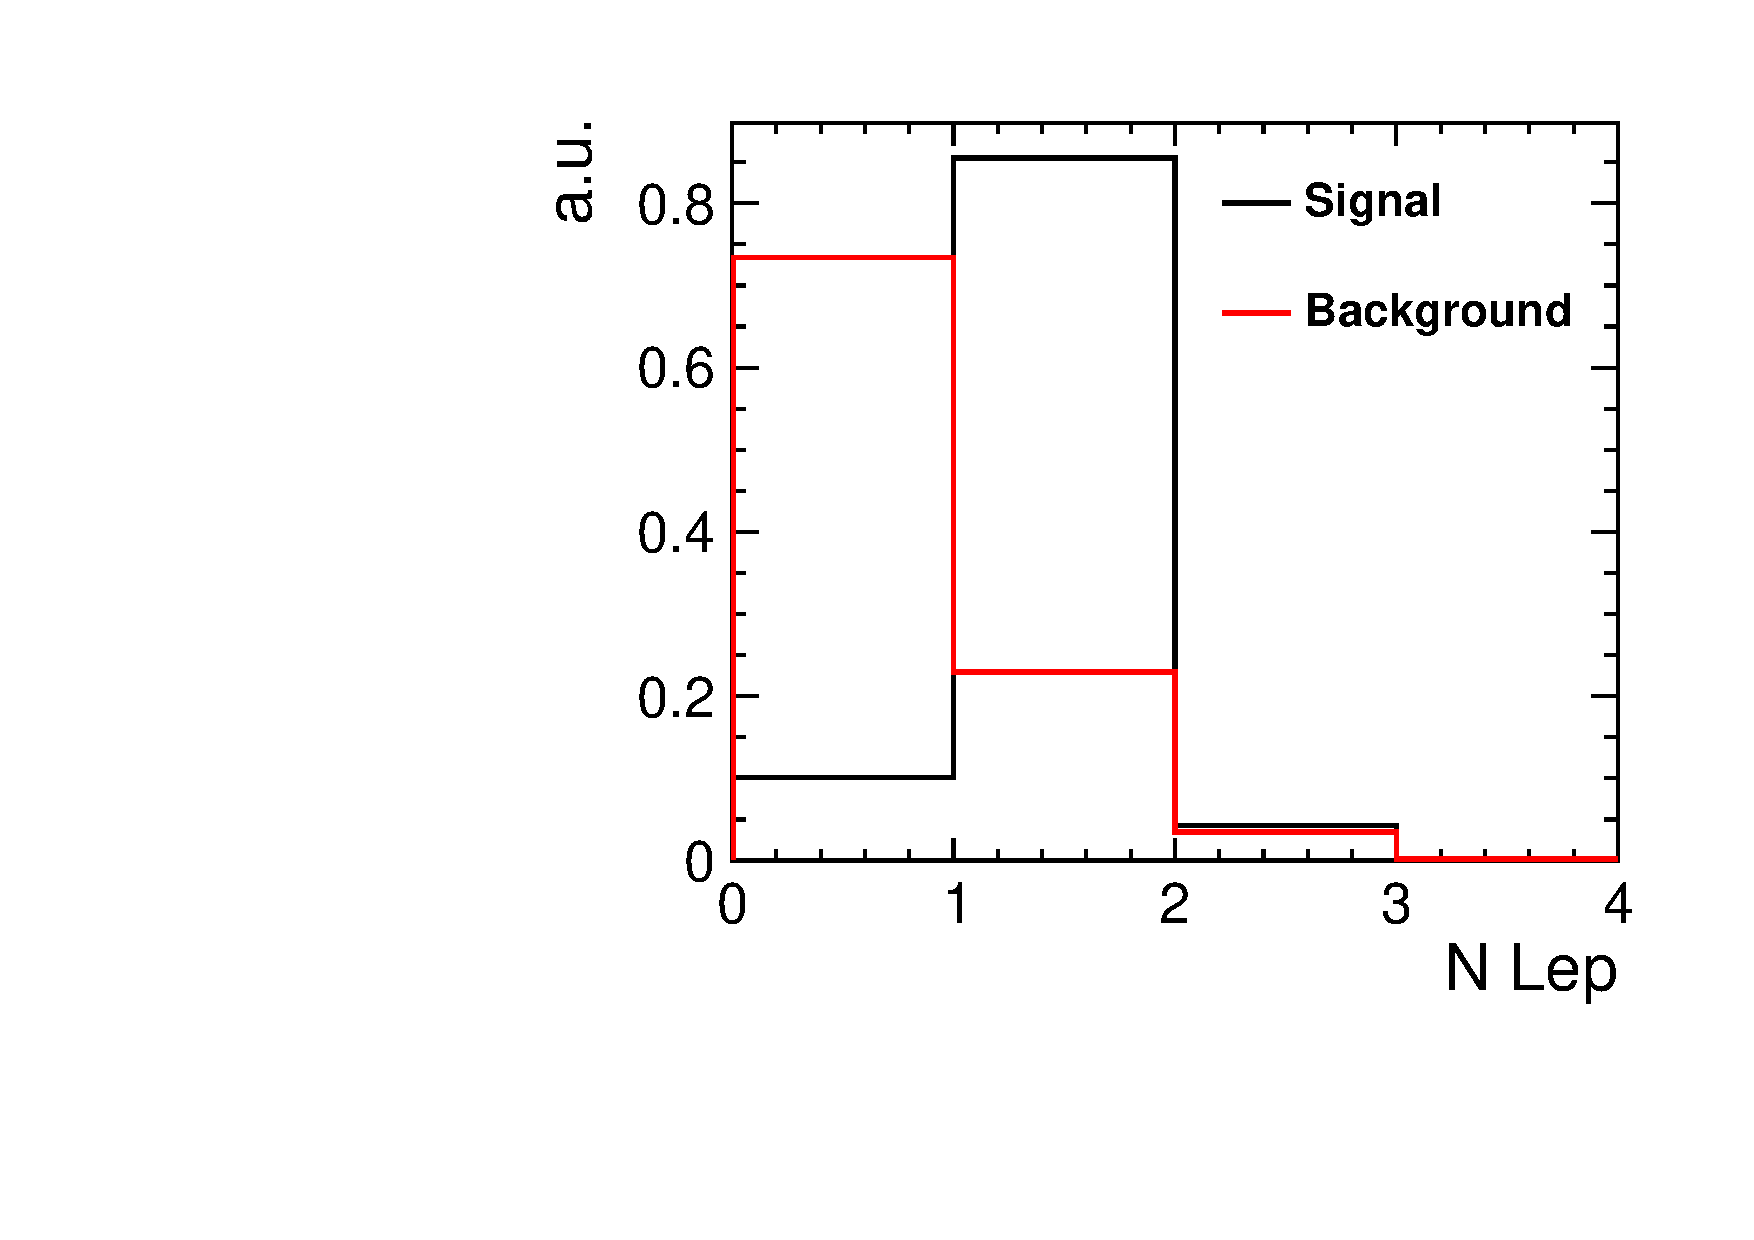
\includegraphics[width=0.75\linewidth]{Appendix/figures/nLep} 
    \caption{Number of reconstructed leptons} 
    \vspace{4ex}
  \end{subfigure}
  \begin{subfigure}[]{0.5\linewidth}
    \centering
    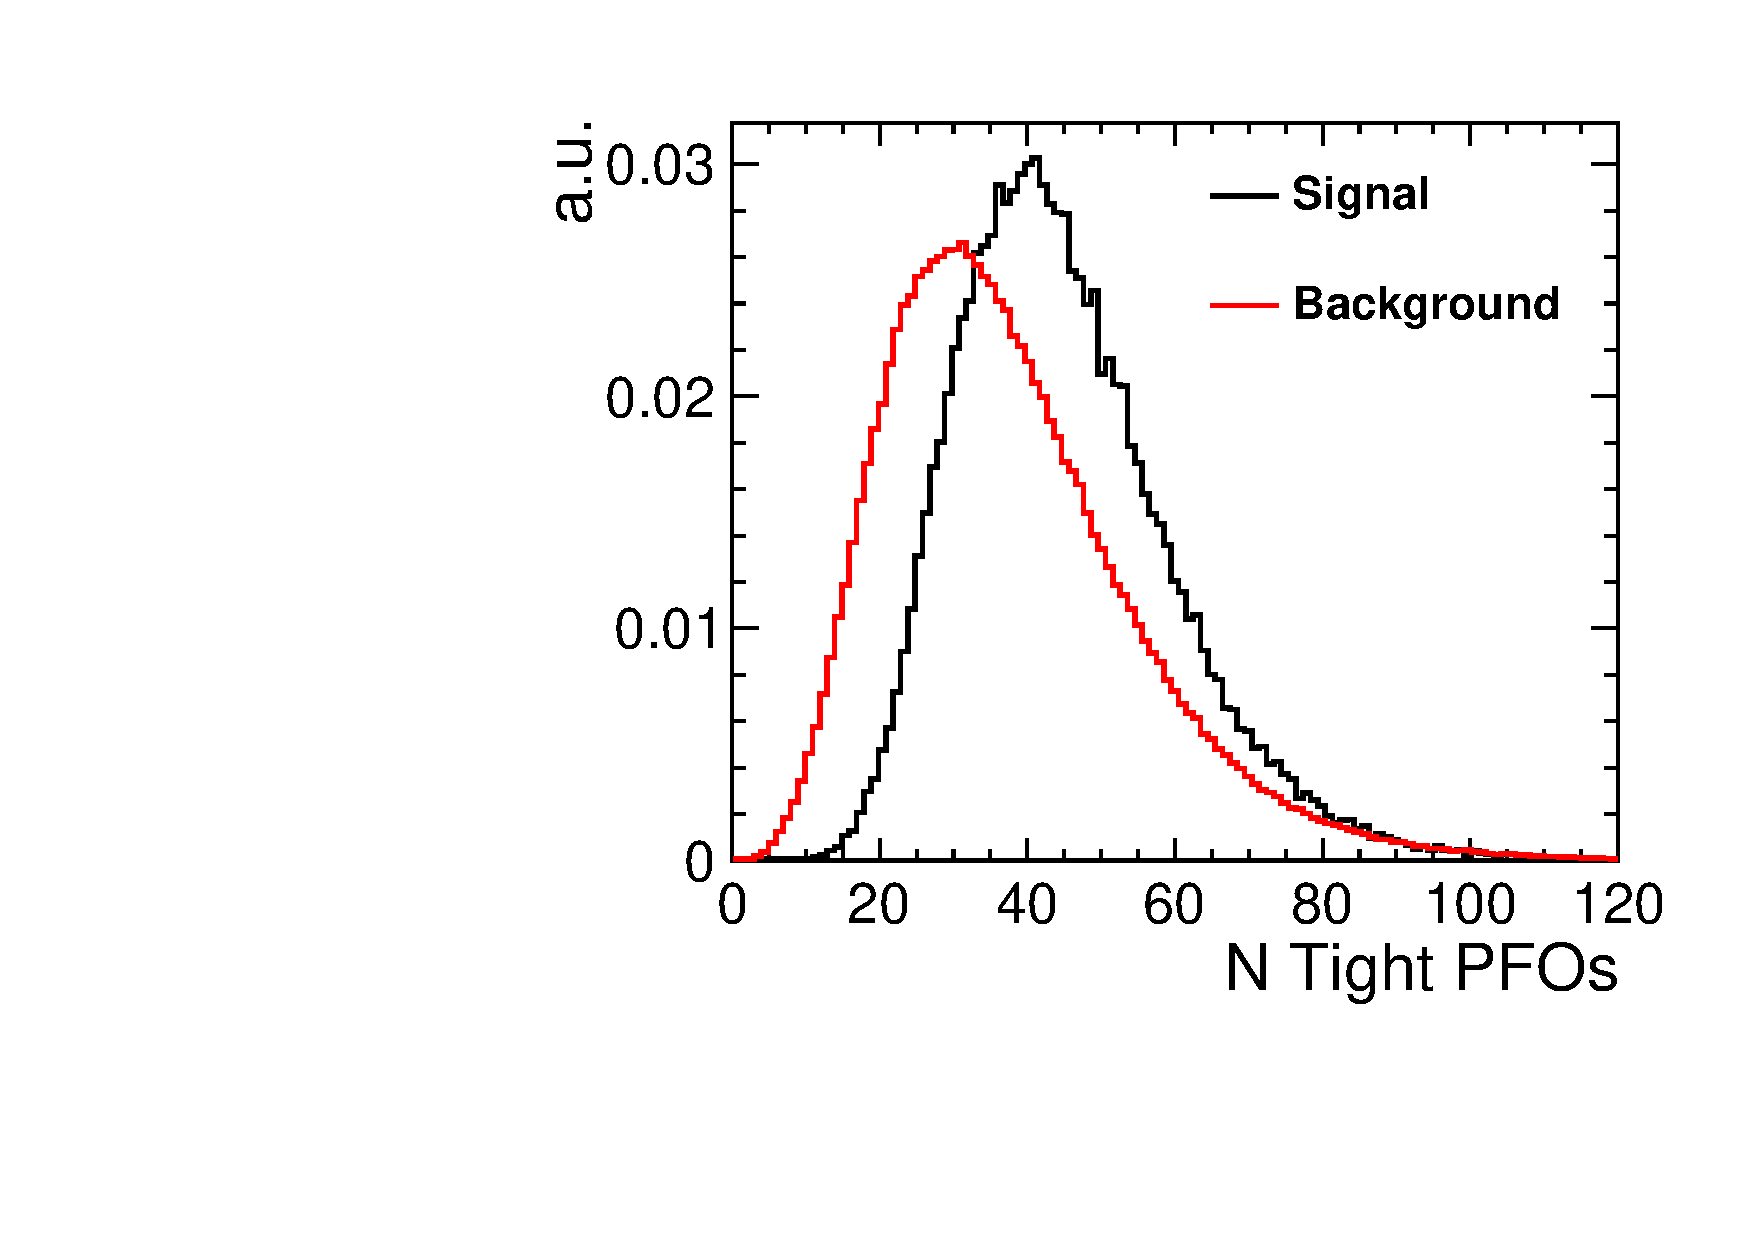
\includegraphics[width=0.75\linewidth]{Appendix/figures/NTightPFOs} 
    \caption{nPFOs passing tight timing cuts} 
    \vspace{4ex}
  \end{subfigure}%% 
  \begin{subfigure}[]{0.5\linewidth}
    \centering
    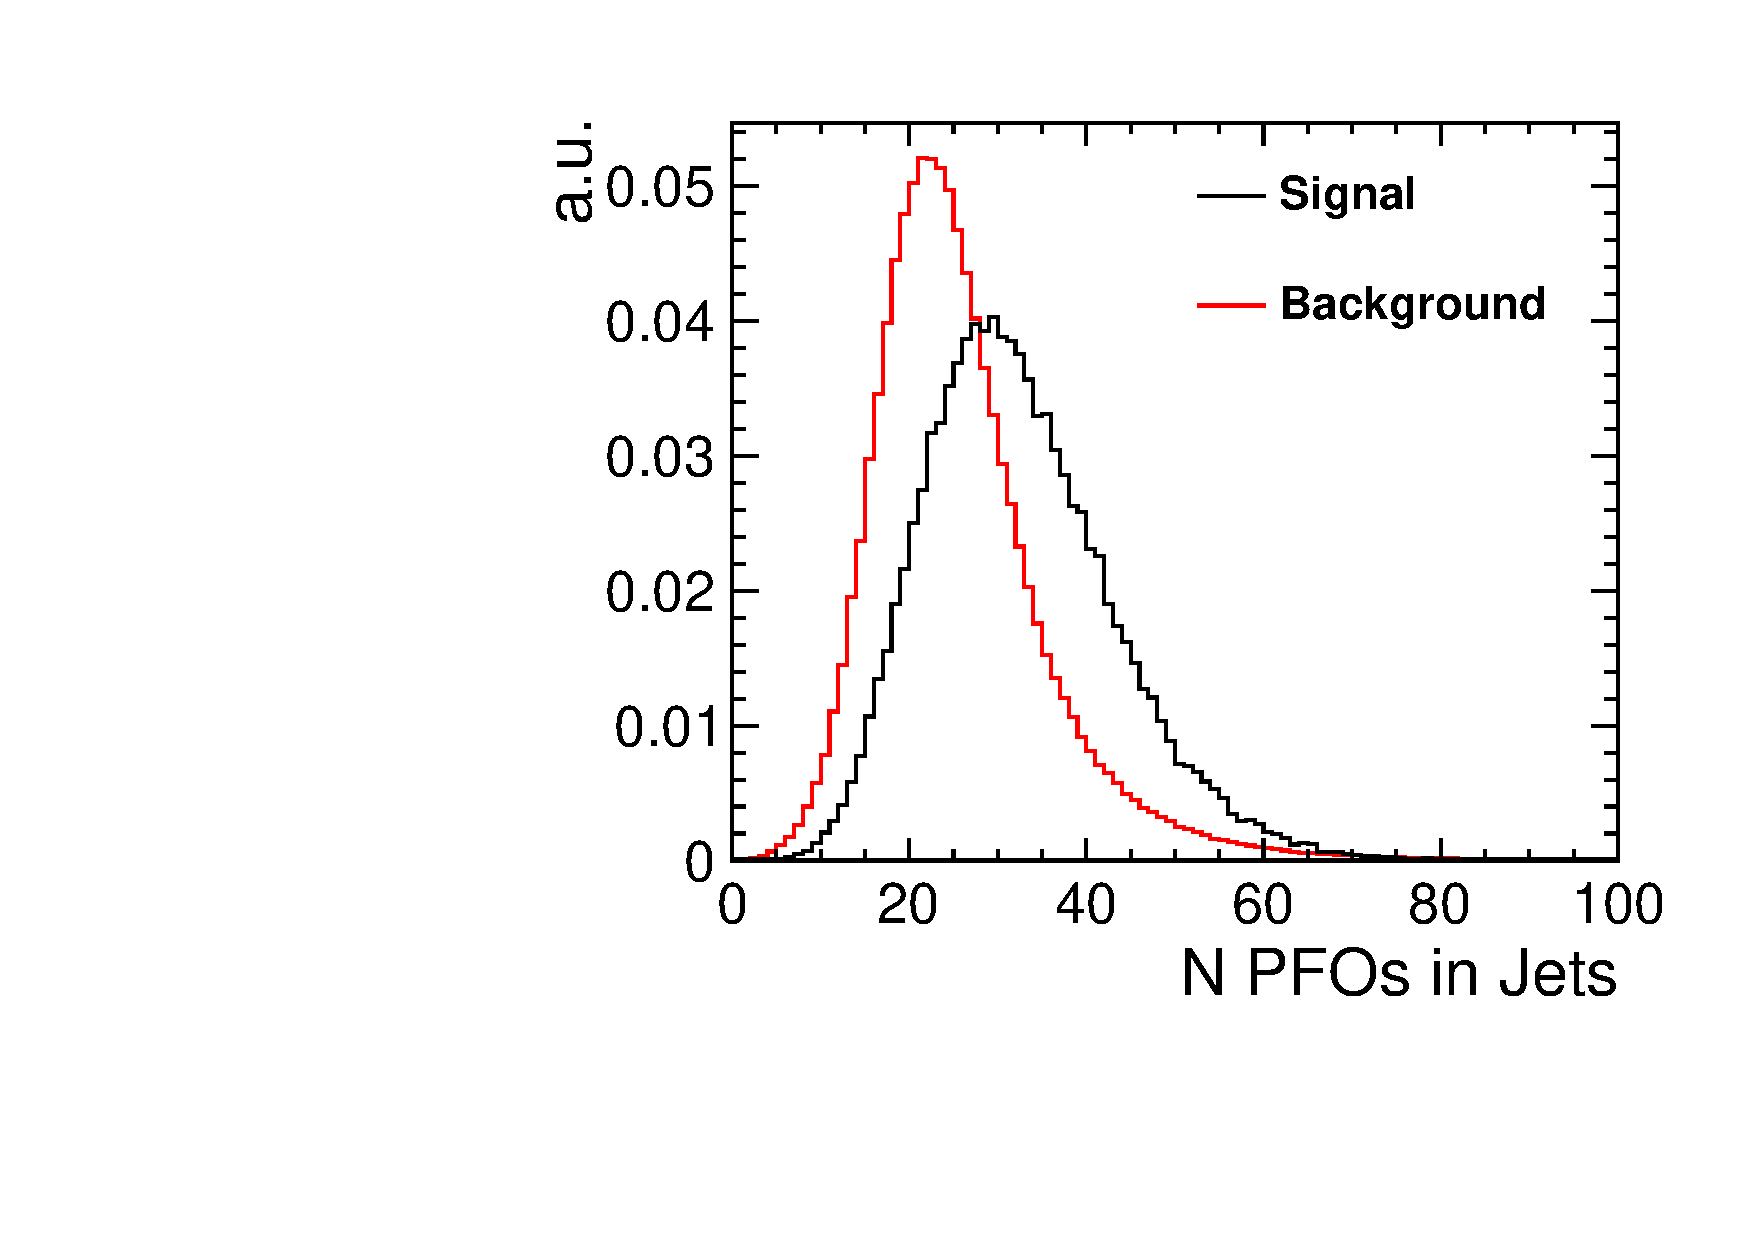
\includegraphics[width=0.75\linewidth]{Appendix/figures/PFOsInJets} 
    \caption{nPFOs assigned to jets} 
    \vspace{4ex}
  \end{subfigure} 
  \begin{subfigure}[]{0.5\linewidth}
    \centering
    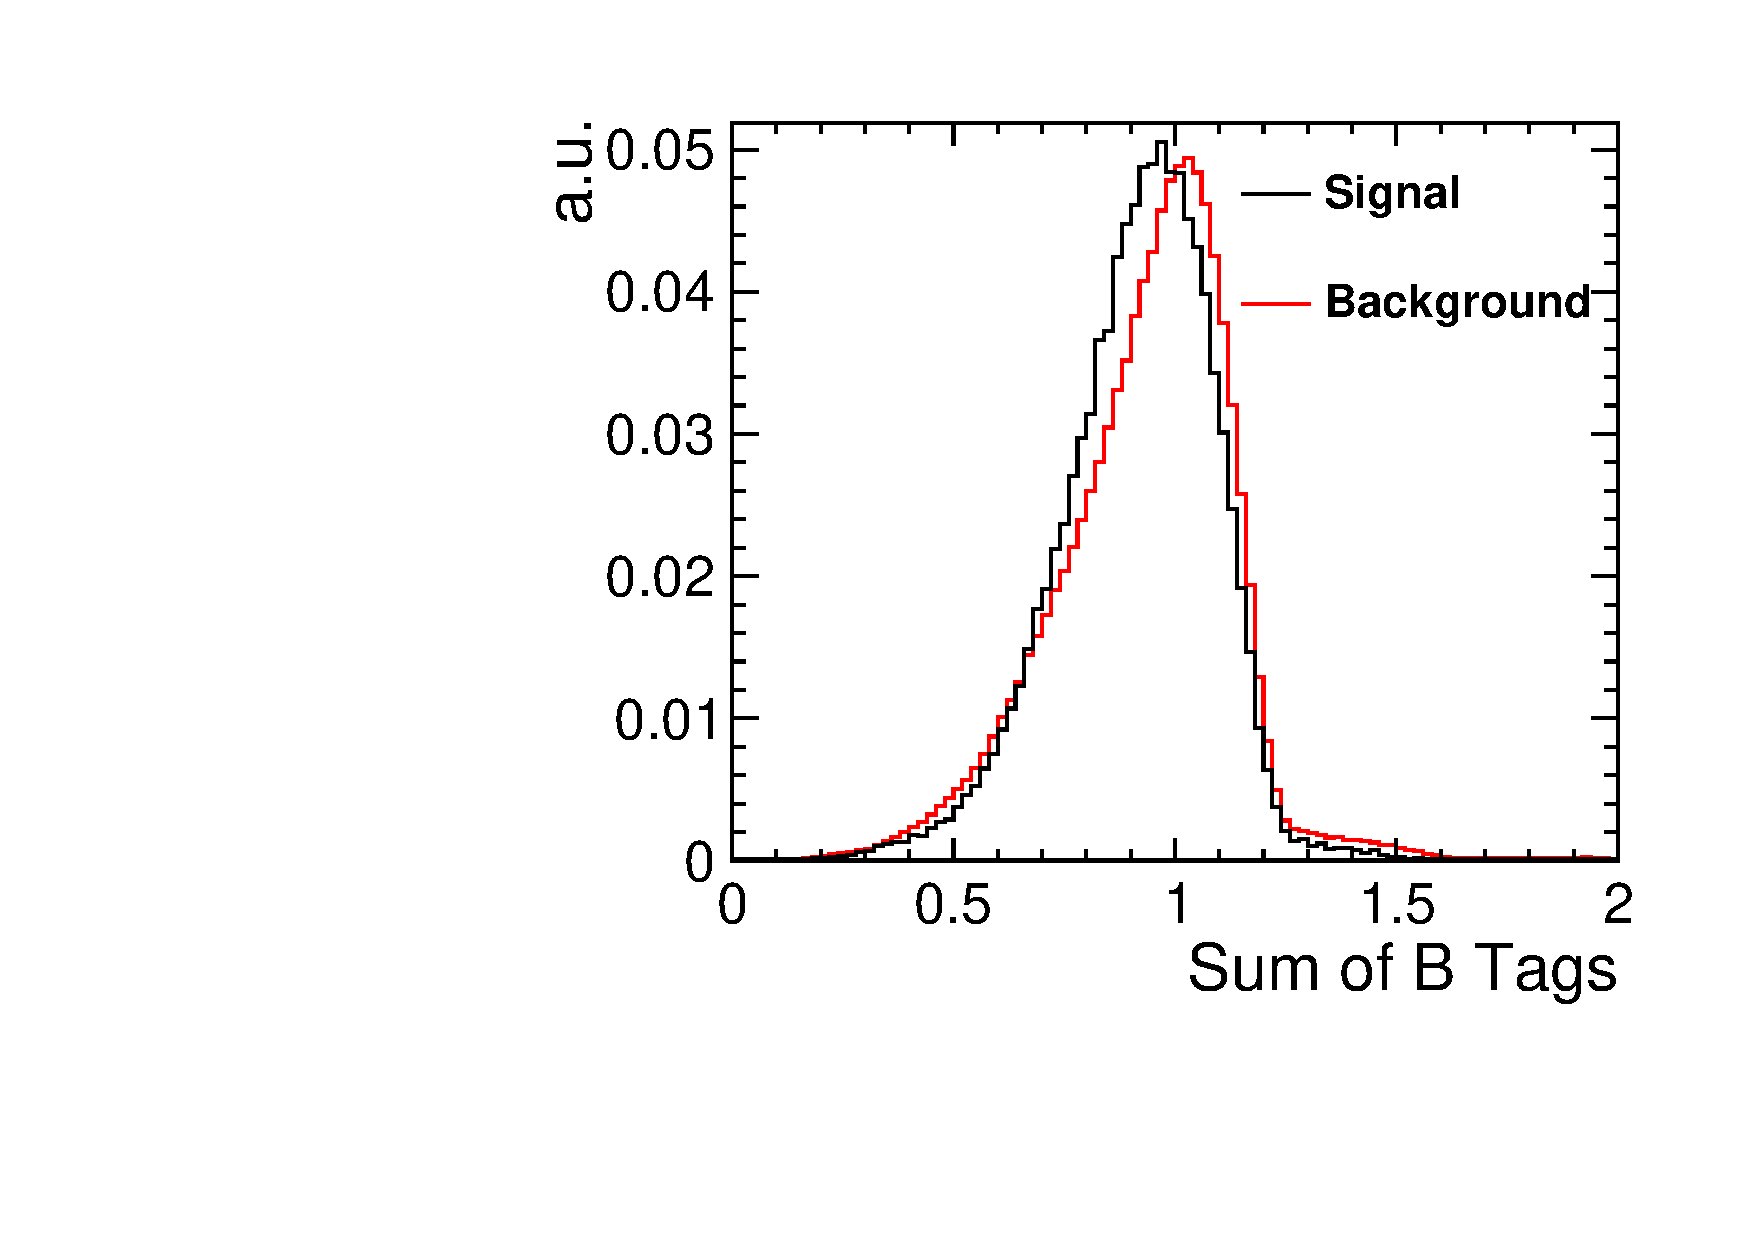
\includegraphics[width=0.75\linewidth]{Appendix/figures/SumBTags} 
    \caption{Sum of two highest b-tags} 
     \vspace{4ex}
 \end{subfigure}%%
  \begin{subfigure}[]{0.5\linewidth}
    \centering
    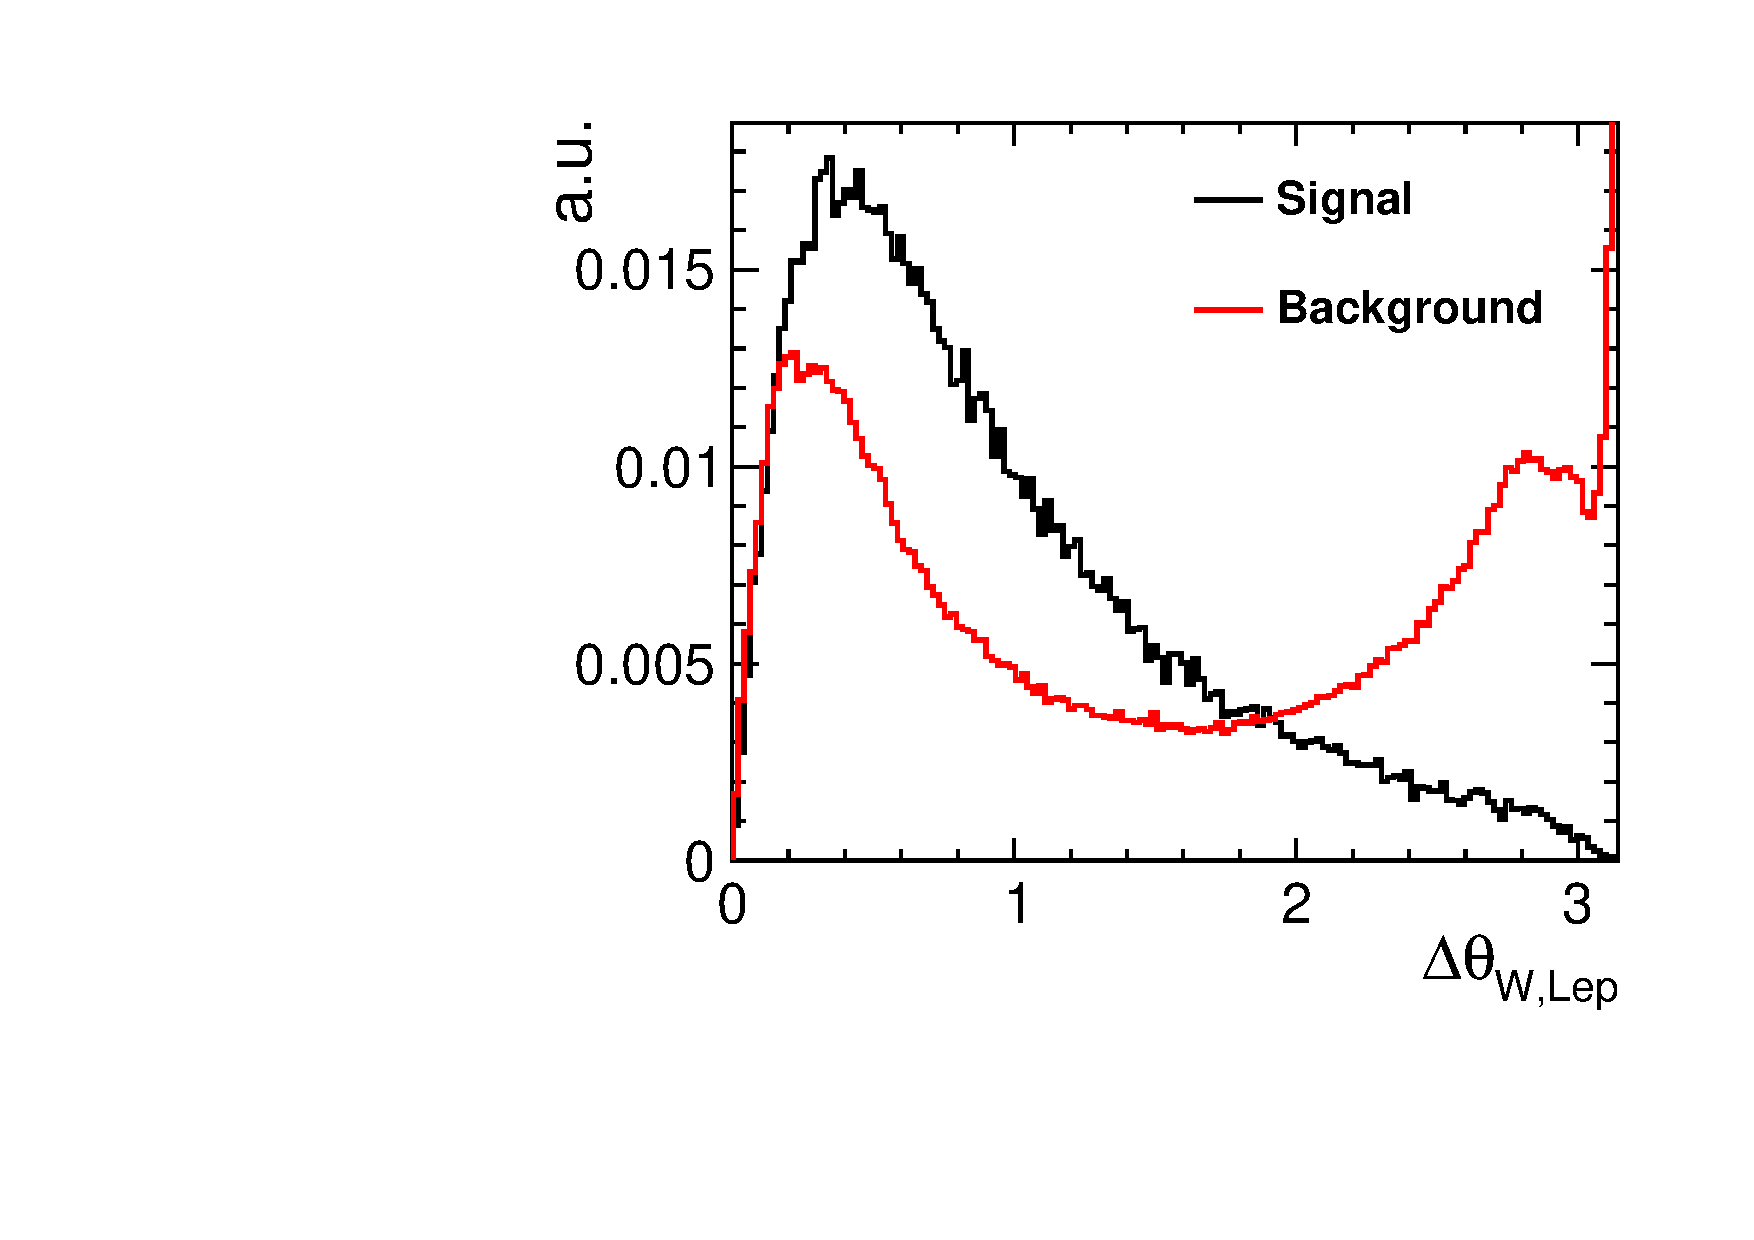
\includegraphics[width=0.75\linewidth]{Appendix/figures/WqqLepAngSep} 
    \caption{Angular Separation of the W and lepton} 
    \vspace{4ex}
  \end{subfigure}
  \begin{subfigure}[]{0.5\linewidth}
    \centering
    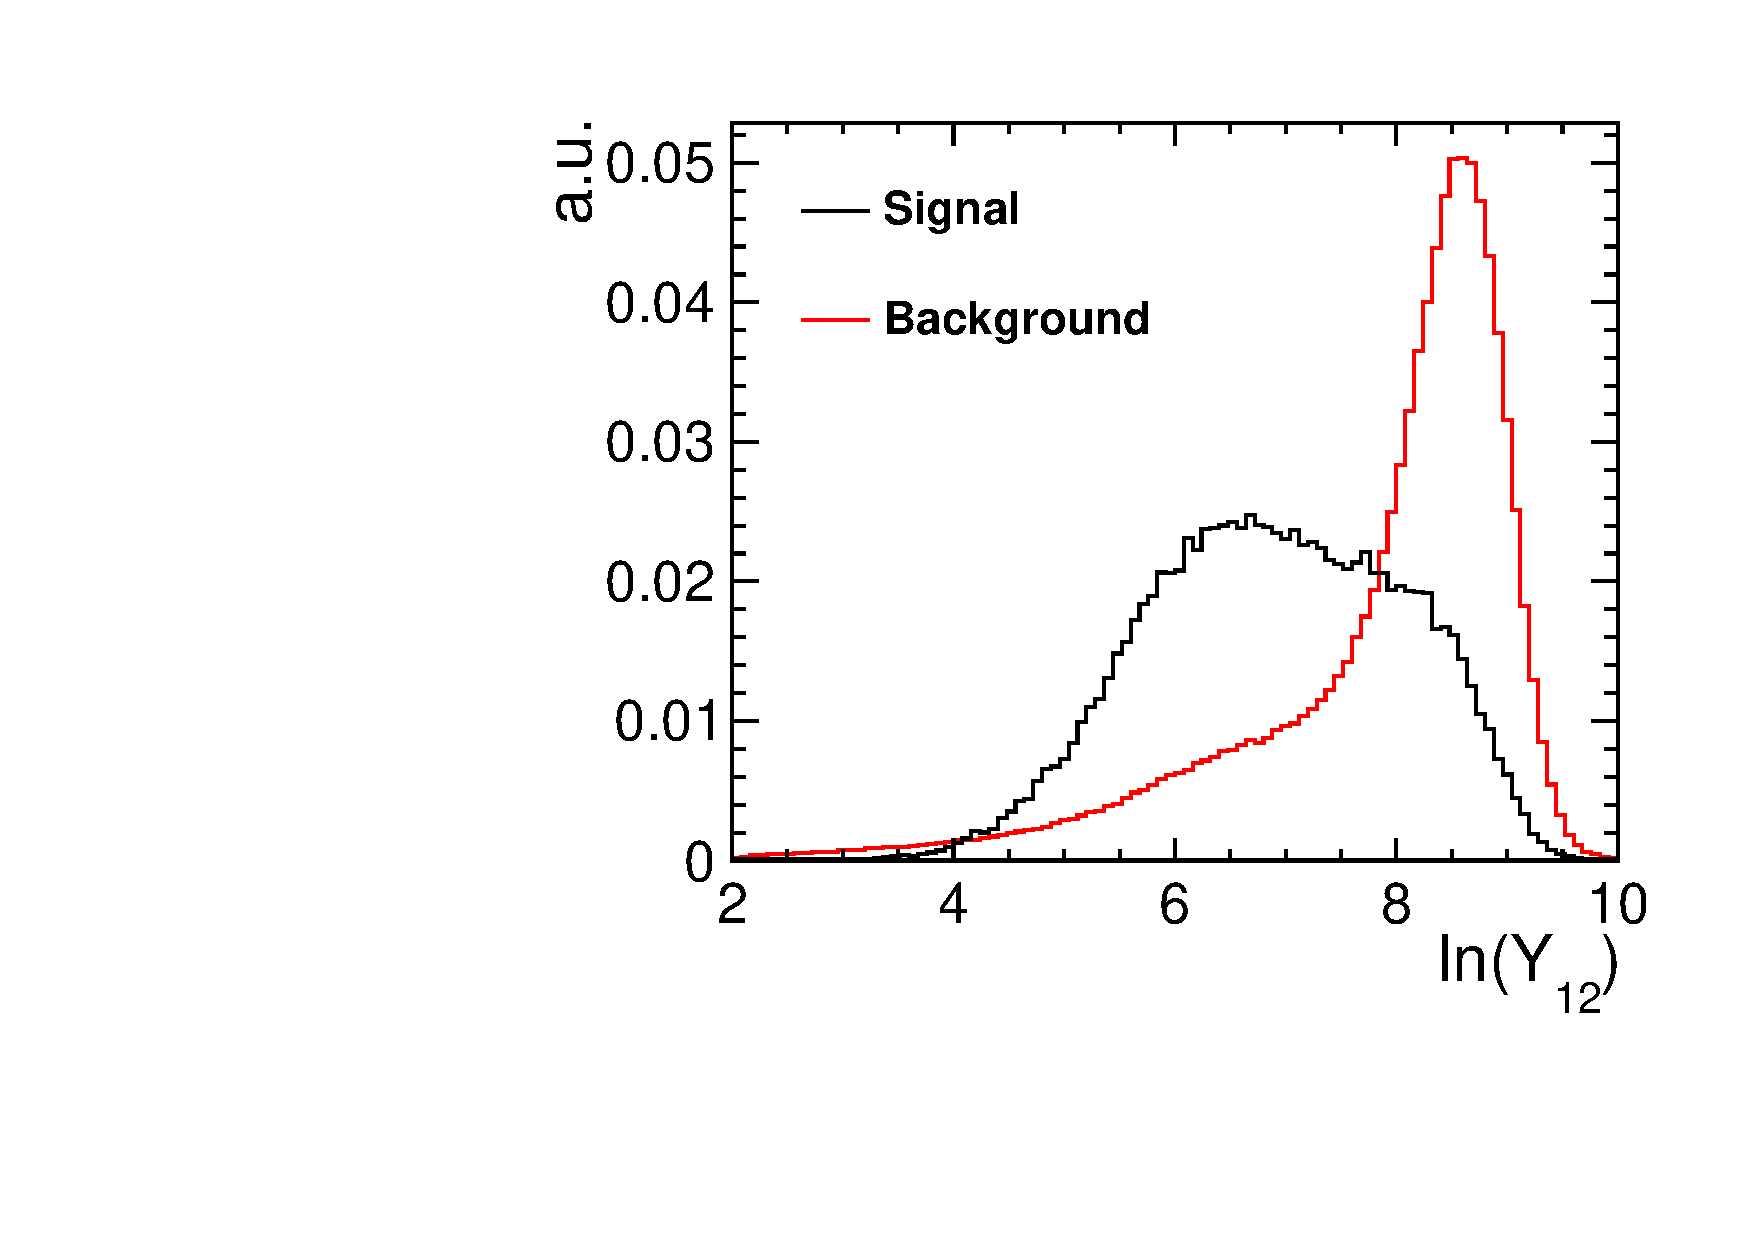
\includegraphics[width=0.75\linewidth]{Appendix/figures/Y12} 
    \caption{Jet Resolution Parameter Y$_{12}$} 
    \vspace{4ex}
  \end{subfigure}%%
\end{figure}


% add references
\printbibliography[title=References]

\end{document}
